% Use only LaTeX2e, calling the article.cls class and 12-point type.

\documentclass[12pt]{article}

\usepackage{times}

\topmargin 0.0cm
\oddsidemargin 0.2cm
\textwidth 16cm 
\textheight 21cm
\footskip 1.0cm

%AMS-Packages .. to be avoided later on.
\usepackage{amsmath}
\usepackage{amsfonts}
\usepackage{amssymb}
\usepackage{graphicx}
\usepackage{color}
%Additional packages
\usepackage{units}
\usepackage{afterpage}
\usepackage{placeins}
\usepackage{hyperref}
\usepackage{booktabs}
\usepackage{multirow}
\usepackage{ragged2e}
\usepackage{tabularx}
\usepackage[mathlines]{lineno}
\linenumbers

% The next command sets up an environment for the abstract to your paper.

\newenvironment{natabstract}{%
\begin{quote} \bf}
{\end{quote}}

% Include your paper's title here

%Maximum title length is 15 words
%\title{Combating global food insecurity with an international wheat reserve}
\title{Combating extremes in global food prices with an international wheat reserve} 
%\title{Improving global food security with an international wheat reserve} 

\author
{C.~Otto,$^{a,d,\ast}$ J.~Schewe$^{a}$, M.J.~Puma $^{b,c,d}$, T.~Falkendahl$^{a}$K.~Frieler $^{a}$\\
  \\
  \normalsize{ $^{a}$Potsdam Institute for Climate Impact Research, Potsdam, Germany}\\
  \normalsize{ $^{b}$The Earth Institute, Columbia University, New York, NY, USA}\\
  \normalsize{ $^{c}$Center for Climate Systems Research and the NASA Goddard Institute}\\
  \normalsize{for Space Studies, New York, NY, USA}\\
  \normalsize{$^{d}$Center for Climate and Life, Columbia University, Palisades, NY, USA}\\
  \\
  \normalsize{$^\ast$Corresponding author; E-mail: christian.otto@pik-potsdam.de} }

% Include the date command, but leave its argument blank.

\date{}


% self defined comments --> to be replaced in final version
\providecommand{\todo}[1]{\leavevmode\newline\textcolor{red}{TODO: #1}}
\providecommand{\av}[2]{\langle #1 \rangle_{#2}}
%\usepackage{xspace}  %leerzeichen bei bedarf, aber nicht vor satzeichen

% Regions
\newcommand{\EUR}{\operatorname{EUR}}
\newcommand{\FSU}{\operatorname{FSU}}
\newcommand{\NAF}{\operatorname{NAF}}
\newcommand{\CPA}{\operatorname{CPA}}
\newcommand{\ROW}{\operatorname{ROW}}

%Units
\newcommand{\mmt}{\,\unit[]{MMT}}
\newcommand{\USD}{\,\unit[]{USD}}
\newcommand{\USDmt}{\,\unit[]{USD\text{ per }MT}}
\newcommand{\bnUSD}{\,\unit[]{bn\,USD}}
\newcommand{\bnbushels}{\,\unit[]{bn\,bushels}}
\newcommand{\Mt}{\,\unit[]{MT}}
\newcommand{\annum}{\,\unit[]{year}}
\newcommand{\bushel}{\,\unit[]{bushel}}
\newcommand{\ts}{\,\unit[]{timestep}}
\newcommand{\minute}{\,\unit[]{min}}

% Acronyms
\newcommand{\RD}{R\&D}

%Mathoperators
\newcommand{\E}{\mathbb{E}}
\newcommand{\argmax}{\operatorname{argmax}}

\newcommand{\secnd}{2^{\operatorname{nd}}}
\newcommand{\third}{3^{\operatorname{rd}}}

%\newcommand{\hPSD}{\hyperlink{PSD}{PSD}\xspace}

\newcommand{\bs}{\boldsymbol}
% expected quantities
\newcommand{\hPi}{\hat{\Pi}}
\newcommand{\hP}{\hat{P}}
\newcommand{\hS}{\hat{S}}
\newcommand{\hD}{\hat{D}}
\newcommand{\ec}{\varepsilon_c}
\newcommand{\hs}{\hat{s}}
\newcommand{\hh}{\hat{h}}

% elasticities
\newcommand{\dce}{\varepsilon^{\operatorname{dc}}}
%final demand
\newcommand{\FD}{\operatorname{FD}}
\newcommand{\Cref}{C^{\operatorname{ref}}}
\newcommand{\Drstar}{D_r^{\star}}
%storage
\newcommand{\Imax}{I^{\operatorname{max}}}
%supplies and WM supplies
\newcommand{\yropt}{\bs y_r^{\operatorname{opt}}}

\newcommand{\bsSROW}{\bs S_{\operatorname{ROW}}}
\newcommand{\SROW}{S_{\operatorname{ROW}}}
\newcommand{\SROWj}{S_{\operatorname{ROW},j}}

%consumer quantities
\newcommand{\Nc}{\mathbb{N}_c}
\newcommand{\Ismaxr}{I^{s,\operatorname{max}}_r}
\newcommand{\Ismax}{I^{s,\operatorname{max}}}
\newcommand{\Is}{I^s}
\newcommand{\Isr}{I^s_r}
\newcommand{\Dmax}{\Delta I^{\operatorname{max}}}
%
\newcommand{\DIcmin}{\Delta I_{\operatorname{c,min}}}
\newcommand{\Ca}{C_{a}}

\newcommand{\hec}{\hat{\epsilon}_c}

%world market prices
\newcommand{\Prstar}{P^{\star}_r}
\newcommand{\Pref}{P^{\operatorname{ref}}}
\newcommand{\Peq}{P^{*}}
\newcommand{\Pc}{P^{c}}
\newcommand{\Pfl}{P^{<}}
\newcommand{\Pceil}{P^{>}}
\newcommand{\Pm}{\langle P\rangle_{15}}

% export restrictions
\newcommand{\erd}{\delta^{\operatorname{er}}}

% spoilage rate
\newcommand{\rl}{r^l}
%stu-ratio
\newcommand{\rstu}{r^{\operatorname{stu}}}
\newcommand{\avrstu}{\langle r^{\operatorname{stu}}\rangle}
% steady state quantities
\newcommand{\starC}{C^{\star}}
\newcommand{\Pmax}{P^{\operatorname{max}}}
\newcommand{\starPmax}{P^{\operatorname{max},\star}}
\newcommand{\starP}{P^{\star}}
\newcommand{\hrstar}{h_r^{\star}}
\newcommand{\starIsmax}{I^{s,\operatorname{max},\star}}
\newcommand{\starrstu}{r^{\operatorname{stu},\star}}
\newcommand{\starm}{m^{\star}}
\newcommand{\starD}{D^{\star}}

%%%%%%%%%%%%%%% 
% timesteps
%%%%%%%%%%%%%%%
\newcommand{\Dt}{\Delta t}
\newcommand{\Tf}{T^f}
%%%%%%%%%%%%%%%
% indices
%%%%%%%%%%%%%%%
\newcommand{\nmax}{n^{\operatorname{max}}}

%%% Local Variables: 
%%% mode: latex
%%% TeX-master: "../amsel_with_optimization"
%%% End: 

%%%%%%%%%%%%%%%%% END OF PREAMBLE %%%%%%%%%%%%%%%%

\begin{document} 

% Double-space the manuscript.

%\baselineskip24pt

% Make the title.

\maketitle 

\begin{natabstract} % not more than 150 words, no citations
High food price volatility on global markets undermines food security. An international grain reserve has been suggested to prevent damaging price extremes, but available modeling approaches do not allow for reliable assessments of its effectiveness under real-world market conditions. Here, we introduce a novel dynamic multi-regional storage model for agricultural markets that accurately reproduces annual world market prices (including the extremes) and regional ending stocks of wheat from 1980 to the present. We demonstrate that an international wheat reserve of 70 million metric tons would have been sufficient to substantially mitigate past price spikes. Critically, its operational costs are estimated to be small compared to the expenses for present national agricultural support programs, meaning that such a reserve could be a viable means to mitigate regional production shortfalls and price-driving national market interventions. As such, it could become an important tool to mitigate the risks of social instability and climate change.
\end{natabstract}

% \paragraph*{One sentence summary} % not more than 125 characters
% Global food security could be enhanced by an international wheat reserve mitigating damaging price extremes at moderate costs.
% \newline
% Main text up to 5000 words

\section*{Introduction}
Crop price volatility on world markets (WMs) is challenging food security especially for poorer consumers in developing and emerging economies \cite{BRA08}, who cannot be protected sufficiently by their local governments \cite{HLPE11}. In just the last decade, two prominent price peaks -– in 2007/08 and in 2010/11 -– are estimated to have pushed 63 \cite{TIW10} to 80 \cite{FAO08} million people and about 44 million people, respectively, into food insecurity. The resulting food riots undermined social stability in multiple countries \cite{BER13}. Highly volatile prices also threaten the income base of producers, especially smallholders \cite{HLPE11} and render hedging and crop insurance for farmers expensive. Long-term investments into agricultural research \& development (\RD) that are key to enhance the resilience of the global food system \cite{GOD10,FED10} are jeopardized.
\todo{Corona and bread basket failures.}

Price volatility results from a complex interplay of various long-term and short-term drivers, whose relative importance is still a contentious topic \cite{TAD14}. The set of long-term drivers discussed to have contributed to the recent global food crises include population growth, changing diets in emerging economies \cite{HEA10}, low investments in \RD~as a consequence of low crop-prices in the 1990s \cite{BRA08}, and, especially in the last decade, the rapidly increasing use of biofuels \cite{GOR13,FRA15}. Short-term drivers include nearly simultaneous droughts affecting several major exporting countries, which led to the record-low stock levels preceding both recent price peaks \cite{TRO11}. In this situation, national policy interventions (such as export restrictions by main producers including the Ukraine and Russia \cite{SHA11} and government-driven restocking attempts by several import depending countries in the Middle East and North Africa and in Asia \cite{TRO11,SCH17}) are discussed to have exacerbated the price hikes by further tightening the WM. Also, some authors argue that the liberalization of future markets in the early 2000s may have created speculative bubbles \cite{TAD14,LAG15}. More process-based quantitative modeling is needed to gain a deeper understanding of the market dynamics \cite{SCH17} allowing for tailored food security policies. 

The recent price hikes have initiated a debate on the benefits of an international grain reserve for global food security. While supported by analyses of the International Food Policy Research Institute \cite{BRA09a}, the High Level Panel of Experts on Food Security and Nutrition of the United Nations (UN) \cite{HLPE11}, the World Bank \cite{LIN08} and the Canadian Foodgrains Bank \cite{MCC11}, its efficacy and feasibility has also been questioned \cite{WRI12}. However, to date much of the existing body of literature provides rather anecdotal evidence \cite{BRA08} or presents findings from highly idealized models \cite{WIL91}, which are not able to reproduce past market conditions and therefore do not allow for quantitative assessments. Consequently, we continue to lack reliable estimates on the necessary reserve capacity and the associated costs.

However, studies on regional reserves show that ....
\todo{Here, we could add the discussion of GOUL}

Here, we introduce an agent-based, dynamic, multi-regional model for agricultural commodity markets that accounts for regional variability of production, commercial and strategic stockkeeping, and unilateral short-term policy interventions such as restocking attempts and export restrictions. The model is designed to quantitatively describe the dynamics of prices and regional stocks with sub-annual resolution.

\todo{Rather intermediate complexity storyline. Short-term component.}

This model is a major advance over widely used competitive storage models \cite{CAF11} and cobweb like models \cite{MIT12}. \todo{This has to be written more equilibrated ... Designed to explain stylized facts of agricultural markets (e.g. skewness and kurtosis of price distributions, these models are unable to quantitatively reproduce either reported prices or regional changes in stocks. Thus, they cannot provide comprehensive assessment of (i) the effectiveness of an international reserve to damp price spikes or (ii) its impact on regional stocks.} Both are key for assessing the effectiveness of a reserve's ability to improve global food security. Further, our model aims to complement large-scale computational (partial) equilibrium models (e.g. the AGLINK-COSIMO model \cite{OECD15} employed by the Food and Agricultural Organization (FAO) of the UN and the Organisation for Economic Co-operation and Development  (OECD)), which are designed to provide long-term price, supply, and demand trends for various socio-economic and climate scenarios. Their complex structure requires a substantial number of modeling assumptions, which renders model validation difficult \cite{VAL07}. Equally important, they are usually calibrated to represent long-term changes in the agricultural system rather than short-term shocks. Together with their coarse (annual to decadal) temporal resolution, the limits their ability to describe price extremes adequately. 


\begin{itemize}
\item \cite{CAF11,GOU13,LAR13,GOU16,GOU16a,KEY38}
\item \cite{Salent paper from 1983}
\item Intro: cite Kais paper , Les16
\item Crop yield variabilty from weather \cite{RAY15}
\item Global crop basket failures \cite{GAU19}
\end{itemize}


We focus our discussion on wheat, arguably the most important food grain. First, we show that our model is able to closely reproduce historical bi-annual world market prices and regional ending stocks from 1980 to the present given reported regional productions, long-term demand trends, and known national market interventions. Then, we use the model to quantify the contributions of different drivers to historical price volatility highlighting the importance of production variability and national policy interventions as main drivers. As these drivers may be difficult to control, we assess the potential of an international reserve scheme as an alternative measure for price stabilization. Such a reserve could be managed, for instance, by a consortium of individual nations together with an international body such as the UN World Food Program (WFP). We discuss policy relevant key aspects such as the reserve's effectiveness in suppressing damaging price extremes and its financial feasibility under real-world market conditions.

A distinguished feature of WMs for agricultural commodities, essential to understand the market dynamics, is the interplay of profit-oriented actors, such as commercial storage holders, with a multitude of governmental policies (such as strategic stockkeeping and import and export levies) aiming to insulate domestic markets from the price volatility at WMs. The latter  largely differ among regions and so does the dependence of domestic consumers upon WM prices. To capture these features, we take a novel modeling approach where we consider (i) five world agricultural regions and (ii) include three representative agents per region: a commercial storage holder, a strategic storage holder, and a domestic consumer.
Price and storage dynamics are determined by the interplay of these regional agents.

\section*{Model}
A detailed model description may be found in Sec.~\ref{si:modDet} of Supplementary Material (SI). The regions accounted for in the simulations include the four largest wheat producing regions (the European Union (EUR), with France and Germany as main producers; the Former Soviet Union (FSU), having Russia and Ukraine as largest producers; the North Atlantic Free Trade zone (NAF), containing the USA and Canada as main producers; and Centrally Planned Asia (CPA), dominated by China with respect to domestic consumption as well as production), and the rest of the world (ROW). 

\paragraph*{Commercial storage holder}
We model the commercial storage holder  as risk-neutral and bounded-rational with a forecast horizon of one year. At each timestep, the agent receives the amount of grain harvested in the region and then plans its next WM supplies by maximizing expected profit over the forecasting period. The latter is calculated from the difference between expected revenues and warehousing costs. Expected revenues depend on the agent's expectation on future WM prices. To form these expectations, the agent estimates (i) its own impact on WM price, (ii) its own harvest in the next year, (iii) the WM supplies of its competitors during this period, and (iv) WM demand. We assume that all commercial storage holders have access to the same global supply and demand forecasts provided, for instance, by the FAO.

\paragraph*{Strategic storage holder}
The strategic storage holder aims at providing food security for the region's domestic consumers. Thus, in contrast to the commercial storage holder, its rationale is not profit maximization, but to assure a target inventory level. The inventory level that is perceived as the optimal tradeoff between food security in times of scarcity and operational costs for warehousing depends on the regional policies and may consequently vary among regions and over time. In the simulations, we assume that the strategic storage holder also encompasses consumer-side stocks at processing firms and wholesalers that are not governmentally owned, but may be regulated by consumer side policies such as import levies and export taxes.

\paragraph*{Domestic consumer}
The third agent type represents the region's domestic consumption. To keep the model simple, we assume that the domestic consumer does not directly purchase grain from the WM, but instead relies on the region's strategic storage. Consequently, this agent's consumption is limited by the content of the region's strategic inventory.  Unless stated otherwise, annual regional consumption is prescribed according to the values reported by the United States Department of Agriculture (USDA). However, for some simulations, we assume an iso-elastically dependence of regional consumption upon WM price. The elasticities of consumption may vary among regions, which accounts for their different dependencies upon the modeled crop.

\paragraph*{Market dynamics}
Price and storage dynamics arise from the interplay of the regional agents at the WM. We assume that the WM clears in each timestep, and the equilibrium WM price is determined by equating WM supply with WM demand.

\paragraph*{Trade policies}
\label{sec:trad_pol}
We consider two types of regional trade policies: policies that directly impact the regions' strategic stocks and export restrictions. The former comprise long-term changes in strategic stockkeeping policies, as well as short-term demand-side responses to tight markets such as restocking attempts and panic purchases\footnote{Further, we assume that other consumer side policies such as import levies can also be represented by changes in strategic stocks.}. These policies lead to temporal changes of the target stocks-to-use (stu) ratio which is perceived as the optimal tradeoff between food security in times of scarcity and the operational costs for warehousing. Consequently, reported changes in regional stu-ratios (calculated from the ratio of ending stocks and domestic consumption) can be considered as indicators for market interventions. For instance, the abrupt decline of the ending stocks in the NAF region between 1986 and 1988 marks the transition from governmentally managed stocks to a market-oriented stockholding scheme \cite{WES99} (see ending stocks and stu-ratio for NAF region in Fig.~\ref{fig:Fig2} and Fig.~\ref{fig:stuRatios} in SI, respectively). We use major regional changes in stu-ratios that can not be solely explained by changes in WM price as proxies for regional changes in the demand for strategic stockkeeping.

Further, we account for major reported national export restrictions by assuming that the region's commercial storage holder is prohibited from selling a certain share of its inventory at the WM. Since export restrictions are short-term policy measures in times of crises, we assume that agents cannot foresee the onset of export restrictions nor their revocation. The affected commercial storage holder  therefore assumes that, once imposed, the restriction will remain in place for the whole foresight period. Since it is not possible to derive the absolute values of both the regions’ strategic storage capacities and the share of inventory that cannot be sold on the WM directly from the trade data, these parameters are determined by the best fit of simulated prices and regional ending stocks with reported prices and stocks (see Sec.~\ref{si:trad_pol} of SI for details on the implementation and Tab.~\ref{tab:tradPol} for a list of the considered policies, their timing, and the reporting sources).

\paragraph*{International reserve}
\label{sec:int_reserve}
The international reserve is a measure designed to reduce price volatility by stabilizing prices within a certain price band centered around a center price, representing long-term price trends. The price band is limited from below by a floor price and from above by a ceiling price. If the price drops below the floor price, the reserve is filled by purchases from the WM until either the price increases above the floor price or the reserve is filled to its capacity. If the price exceeds the ceiling price, grain is released from the reserve onto the market until either the price drops below the ceiling price or the reserve is depleted.

\paragraph*{Results}
We model biannual WM prices and regional inventory dynamics for wheat from 1980 to the present. The model is driven by annual production data from the USDA, which are combined with regional crop calendars to determine each region's harvesting season (see Sec.~\ref{si:MM} of SI for details). Accounting for the main regional storage policies reported in the literature (Tab.~\ref{tab:tradPol} in SI), we are able to closely reproduce reported prices and ending stocks as indicated by high squared Pearson correlation coefficients $R^2$ (Figs.~\ref{fig:Fig1} and \ref{fig:Fig2}).

We model biannual WM prices and regional inventory dynamics for wheat from $1980$ to the
present. The model is driven by annual production data of the USDA, which are combined with regional
crop calenders to determine each region's harvesting season (see Secs.~\ref{si:MM} of SI for details). Accounting for the main regional storage policies reported in
the literature (Tab.~\ref{tab:tradPol} in SI), we are able to closely reproduce reported prices and
ending stocks as indicated by high squared Pearson correlation coefficients $R^2$
(Figs.~\ref{fig:Fig1} and \ref{fig:Fig2}).

\paragraph{Main drivers of price volatility}
Forcing the model solely by long term variations in production and demand (`trends only scenario')  demonstrates that only 0.2\% of the observed variance in prices can be explained by these drivers. After removing the long-term trends in the simulated and observed time series by taking first differences, no variance can be explained at all. Accounting for annual fluctuations in regional production and consumption (`production \& consumption variability' scenario), the explained variances increases to 14.7\% and taking historical policy interventions into account (“full historical scenario”) allows for 79.2\% of the variance to be explained (see Sec.~\ref{si:scen} of SI for detail on the different scenarios). After detrending, the explained variance for the 2\textsuperscript{nd} scenario (34.3\%) is nearly as high as for the full historical scenario (36.3\%) showing that, for the years 1980 to 2017, short-term fluctuations of production and consumption were by far the dominant drivers of the short-term price volatility at the wheat market. In contrast, strategic long-term decisions on the management of stocks have mainly contributed to the decaying price trend from the 1980s to 2006 (cp. also Fig.~\ref{fig:baseline} in SI to Fig.~\ref{fig:Fig1}). This is why the explained variance (without de-trending) is much higher for the full historical scenario than for the 2\textsuperscript{nd} scenario not accounting for trade interventions. We find that short-term policy responses such as restocking attempts and panic purchases of import dependent MENA countries (ROW region) as well as China (CPA region) have significantly contributed to the 2007/08 and 2010/11 price spikes, which is in line with previous works \cite{HEA08,TRO11,HEA10}. In a scenario without policy changes after 2006 (Figs.~\ref{fig:prices_small_res} and \ref{fig:stocks_small_res} in SI), price spikes are strongly suppressed compared to the full historical scenario. Further, by studying a scenario without export restrictions (Figs.~\ref{fig:prices_small_res} and \ref{fig:stocks_small_res} in SI), we find that export restrictions are crucial to match post-2006 regional ending stocks, but less important than restocking attempts and panic purchases as driver of price volatility.

The overall good fit obtained by accounting only for observed regional fluctuations of consumption
and production and national trade interventions suggests that, on a biannual timescale, supply and
demand dynamics have been the dominant drivers of WM price fluctuations; cross-markets
interactions and speculative bubbles have played a subordinate role. However, we cannot rule out
that the latter become more important on daily to monthly time-scales as suggested by
\cite{LAG15}. Our results are in good agreement with the findings of an earlier study using a global,
dynamic storage model with an annual timestep \cite{SCH17} and show that the conclusions of this
study remain valid in a multi-regional setting and for a biannual timescale.

\paragraph*{Effectiveness of international reserve}
The proposed management scheme for the international reserve is effective; even under the `worst-case' assumption that the reserve cannot mitigate price driving national policy interventions (such as the reported beggar-thy-neighbour policies), infrequent price extremes are efficiently suppressed. In the full historical scenario, a reserve of 70 million metric tons (MMT) would have suppressed the most prominent price spike in 2006/07 by 26\% (Fig.~\ref{fig:Fig1}). Because in this scenario, production and consumption in each region are fixed to their reported values, the build-up of the reserve cannot be modeled; it would create an additional demand that cannot be compensated for by production or consumption responses over time. This is why, we initiate the simulations with a filled reserve (Fig.~\ref{fig:Fig2} (global)). However, the reserve remains effective even when accounting for its build-up in a setting where regional consumptions depend iso-elastically on price (see Sec.~\ref{si:scen} of SI for details).  During this build-up, prices increase due to the additional demand of the reserve, but the resulting reductions of regional consumption are modest. Moreover, regional ending stocks are only slightly reduced, suggesting that the reserve's build-up has a negligible impact on the food security of vulnerable consumers (Fig.~\ref{fig:varDem_cons} in SI).

To quantify the reserve's effectiveness in the long-run and under a range of different production conditions, we also drive the model with a 10,000-year artificial production time series that mimics the historic distribution of production anomalies in each region. The size of the strategic inventories is derived from the average observed stu-levels of the international trade years\footnote{According to the definition of the USDA, the international trade year for wheat spans from July to June of the following year.} 2010 to 2015 (see Sec.~\ref{sec:artiTs} of SI for details). Initially, the reserve is empty; the width of the price band of 18\USD~is chosen to optimally suppress prices above the 90\textsuperscript{th} percentile (prices $P\geq 93$\USD) of the price distribution for the full historical scenario. Infrequent price extremes are strongly suppressed by the reserve (thinning of the tails of the price distributions in Fig.~\ref{fig:Fig3}\textbf{A}), whereas overall volatility (measured by the standard deviation of the detrended time series) is only moderately reduced (Fig.~\ref{fig:Fig3}\textbf{B}). The probability of the occurrence of damaging price hikes (here defined as $P\geq 93$\USD) is already strongly reduced for a reserve with a capacity of 30\mmt~(Fig.~\ref{fig:Fig3}\textbf{C}).

\section{Discussion}
It is worth noting that in all scenarios, price volatility, albeit reduced, is not strongly suppressed for two reasons: (i) the reserve remains passive when prices stay within the (broad) price band, and (ii) the floor price is not defended at all costs; if the reserve is filled to its capacity, no more grain is purchased at the market. This is crucial, because price signals set incentives for producers to invest into \RD. They also foster national attempts to enhance food security increasing the overall resilience of the food system \cite{HLPE11}; preservation of some price variability is essential, otherwise we may risk creating a more fragile global food system \cite{TAL12}.

To evaluate the reserve's feasibility, we relate the necessary reserve size to the capacity of existing storage facilities. Data on storage capacities are difficult to obtain on a national level, because many countries, e.g, China and India, consider information on grain stocks to be sensitive. However, for the US, estimates on total storage capacities for all grains are provided by USDA's National Agricultural Statistics Service. For 2012, stock capacity was estimated at 23.16\bnbushels \cite{NASS14} (504\mmt~wheat equivalent\footnote{The conversion factor for wheat is
  $1\bushel\, \hat{=}\, 0.021772\Mt$ according to
  \url{http://www.grains.org/buyingselling/conversion-factors}.}). Thus, a 70\mmt-reserve would require additional storage capacity corresponding to about 14\% of the present US reserve capacity. If this burden were shared among many countries as suggested by Justin Lin, the World Bank's former vice president \cite{LIN08}, each country would have to increase its storage capacity only by a small fraction.

Reliable estimates of the reserve's financial viability are key to avoid it becoming a major financial drain, hampering much needed investment in \RD~\cite{WRI12}. Early simulations using a stylized competitive storage model suggested that the reserve may pile up huge stocks of grain in times of abundance entailing unsustainable costs for storage operation \cite{WIL91}. In the reserve management scheme discussed here, the build-up of stocks is limited by the reserve's finite capacity. With annual operational costs of grain storage in industrialized countries ranging between 15 \cite{WIG09} and 36\USDmt~\cite{THO10}\footnote{These costs estimates comprise fixed
  costs such as costs for facility construction and operation and variable costs depending upon
  tonnage including costs for drying grain and grain wastage. Following estimates of the Grains
  Research \& Development Corporation of the Australian Government
  (\url{https://grdc.com.au/archive/key-issues/economics-of-storing-grain/details}, accessed June,
  2017), we assume annual fixed cost of 5\USDmt.}, we estimate annual operational costs for a 70\mmt-reserve to be between 0.7 and 1.4\bnUSD. These numbers are obtained from the simulation with iso-elastic demand accounting for all policies (cf.~Figs.~\ref{fig:varDem_price}--~\ref{fig:varDem_cons} in SI), and they are confirmed by our statistical analysis (Fig.~\ref{fig:Fig3}\textbf{C}). Although substantial, they are still small compared to the costs of present national agricultural support programs. For instance, they would make up only between 0.7\% and 1.5\% of the annual expenses for the latest US Farm Bill, the Federal Agriculture Reform and Risk Management Act of 2013 (with projected total costs of 956\bnUSD~in ten years to be spent mainly on producer and consumer support such as crop insurance and supplemental nutrition). Further, the co-benefits of a reserve could compensate for some of these costs. First, by dampening price spikes, it would reduce the expenditures needed to directly respond to food emergencies, reducing the burden of the WFP and other national and non-governmental initiatives. Second, by dampening overall price volatility, it would ensure more stable incomes for farmers and lower their expenses for crop insurance. As a result, other farm support programs could possibly be reduced. Further, it appears reasonable to assume that the trust of market participants in the security provided by a reserve would reduce beggar-thy-neighbour politics and panic purchases, at least to a certain extent. For instance, in a `best-case'-scenario where policy changes are eliminated from 2006 onwards, already a reserve of 30\mmt~would have substantially suppressed the recent price spikes, which is consistent with our findings from the statistical analysis (Fig.~\ref{fig:Fig3}\textbf{B})).

Ongoing climate change may increase production variability \cite{WHE13} and may render nearly simultaneous crop failures in major production regions, like those that substantially contributed to the two recent world food crises \cite{ASS11,CHA14}, more likely. Consequently, damaging price extremes may become an increasingly urgent threat for global food security in the future. The international wheat reserve management scheme presented here could be a viable means to mitigate price volatility, potentially complementing efforts to impede beggar-thy-neighbor policies by binding international free-trade legislation suppressing export restrictions \cite{ANA13}. Both measures require international trade cooperation. Prolonged failure of the WTO to make progress on the Doha Agenda sows doubts that substantial progress on international trade agreements will be made anytime soon in this forum \cite{HLPE11}. Therefore, it appears advisable to follow a two-pronged strategy: if no progress can be made in the WTO negotiations, an international reserve can still be implemented by a different multi-national association that comprises the main producing countries such as the UN or the Organization for Economic Cooperation and Development.

\section*{Methods}%Maximum of 3000 words

\bibliographystyle{naturemag}
\bibliography{lib}


\section*{Acknowledgments}
The authors would like to thank Peter de Menocal for in-depth discussions and
helpful comments. The work was supported by the Leibniz Competition
(SAW-2013-PIK-5), by the German Federal Ministry of Education and Research
(BMBF) under the research project SLICE (FKZ: 01LA1829A) and has received
funding from the Center for Climate and Life as well as the Initiative on
Extreme Weather and Climate of Columbia University, New York, NY.  \todo{World
  Modelers, RECEIPT}

\begin{figure}[htbp]
  \centering
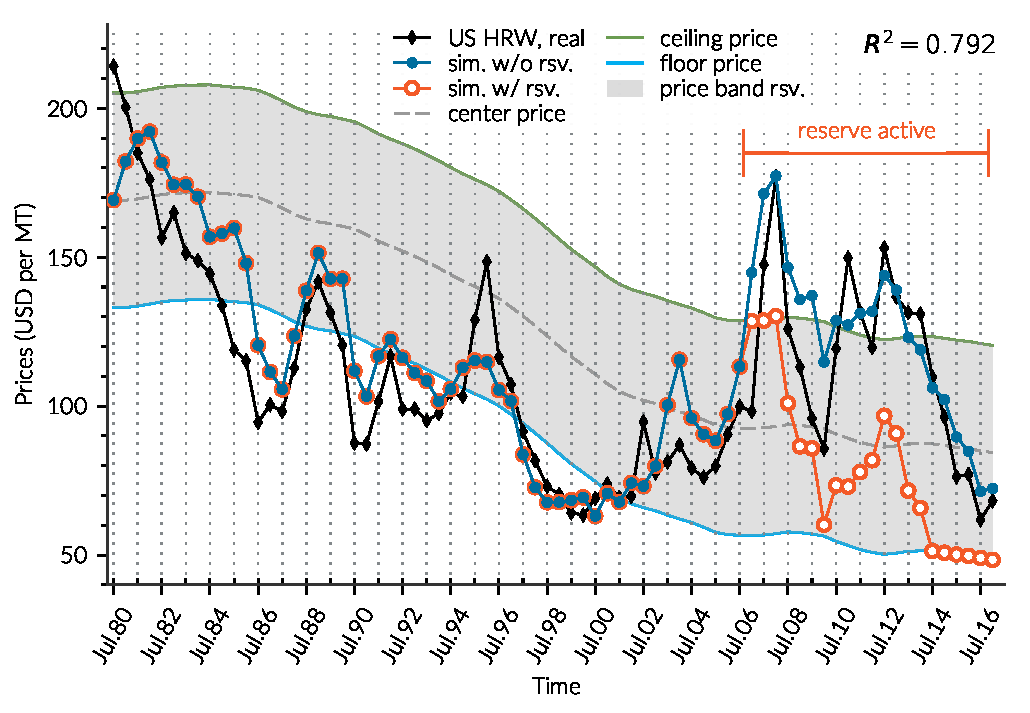
\includegraphics[width=.8\textwidth]{plots/full/pric1980_2017}
\caption{Time series of real wheat prices (black diamonds), simulated prices without (blue dots) and with international wheat reserve (open orange circles). The gray shaded area indicates the reserve's price band which has a width of 70\USD; the reserve is restocked (released), if prices drop below (increase above) the floor price (thin light-blue line) (ceiling price (thin green line)). The price band is centered around the mean price of the previous 15-years (gray dashed line). Correlations between reported and simulated prices (w/o reserve) are measured by the squared Pearson correlation coefficient $R^2$. The orange bracket marks the time span where the reserve actively impacts on market dynamics.}
\label{fig:Fig1}
\end{figure}
\begin{figure}[htbp]
  \centering
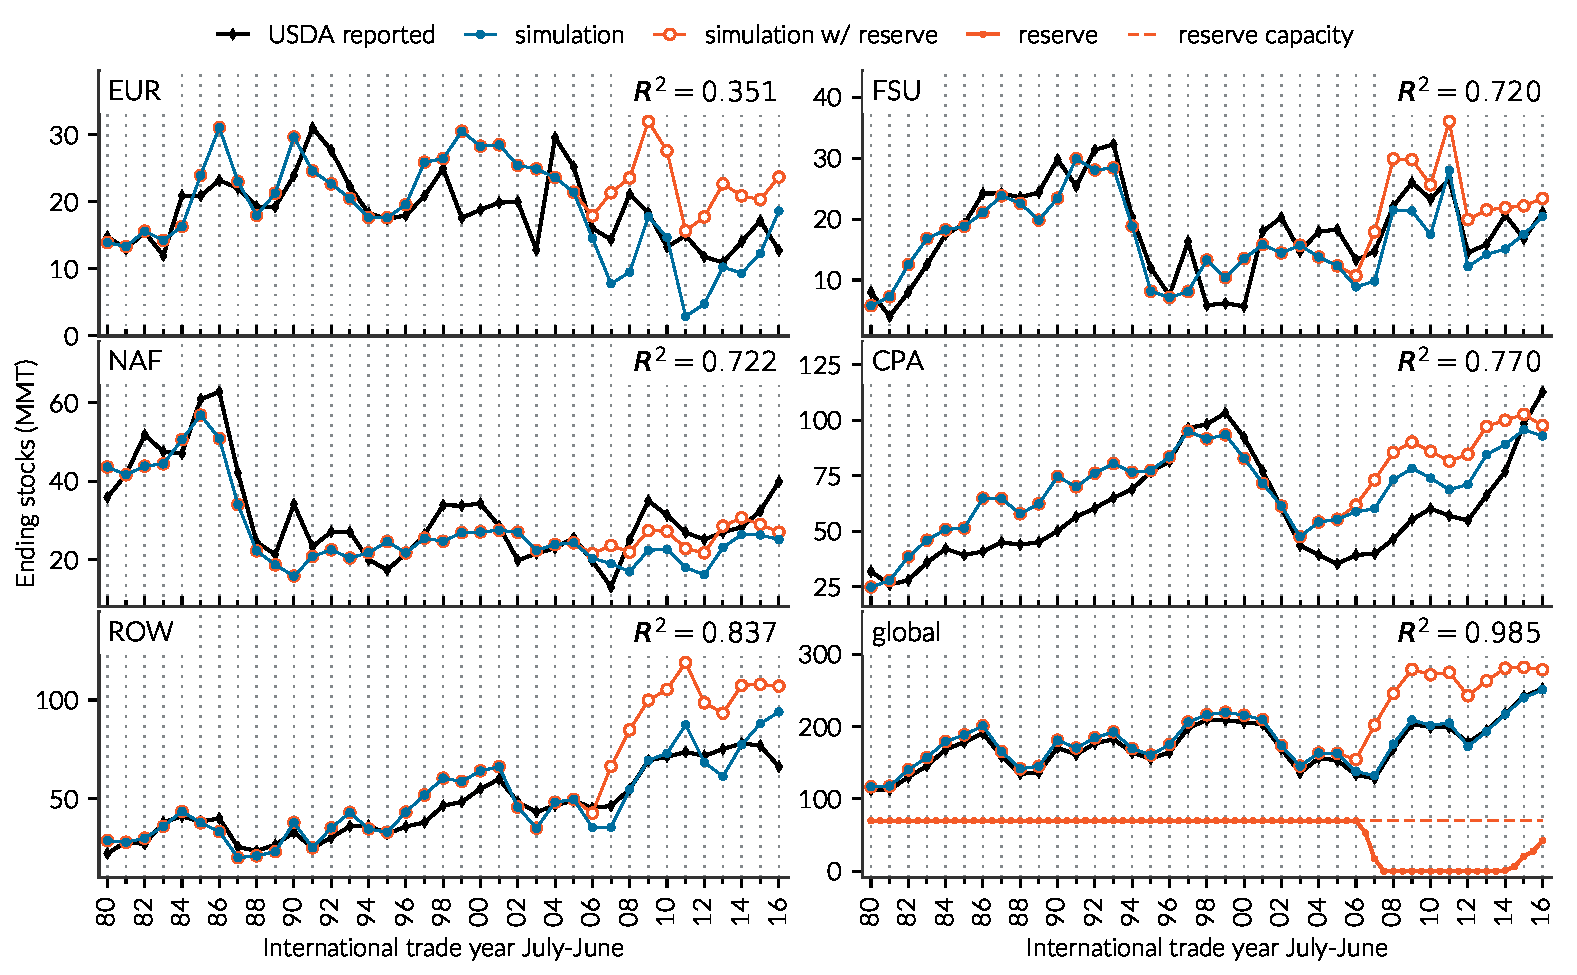
\includegraphics[width=.8\textwidth]{plots/full/Ending_stocks__MMT__1980_2017}
\caption{Ending stock for the five agricultural regions: European Union (EUR), Former Soviet Union (FSU), North Atlantic Free Trade countries (NAF), Centrally Planned Asia (CPA ), rest of the world (ROW), as well as global stocks (global). Black diamonds indicate ending stocks as reported by USDA, and blue dots and open orange circles indicate simulated endings stocks without and with international wheat reserve, respectively. Squared Pearson correlation coefficients $R^2$ denote the correlation between reported stocks and the simulation without reserve. In `global', tonnage and capacity of the international reserve are indicated by small orange dots and an orange line, respectively.}
  \label{fig:Fig2}
\end{figure}
\begin{figure}[htbp]
\centering  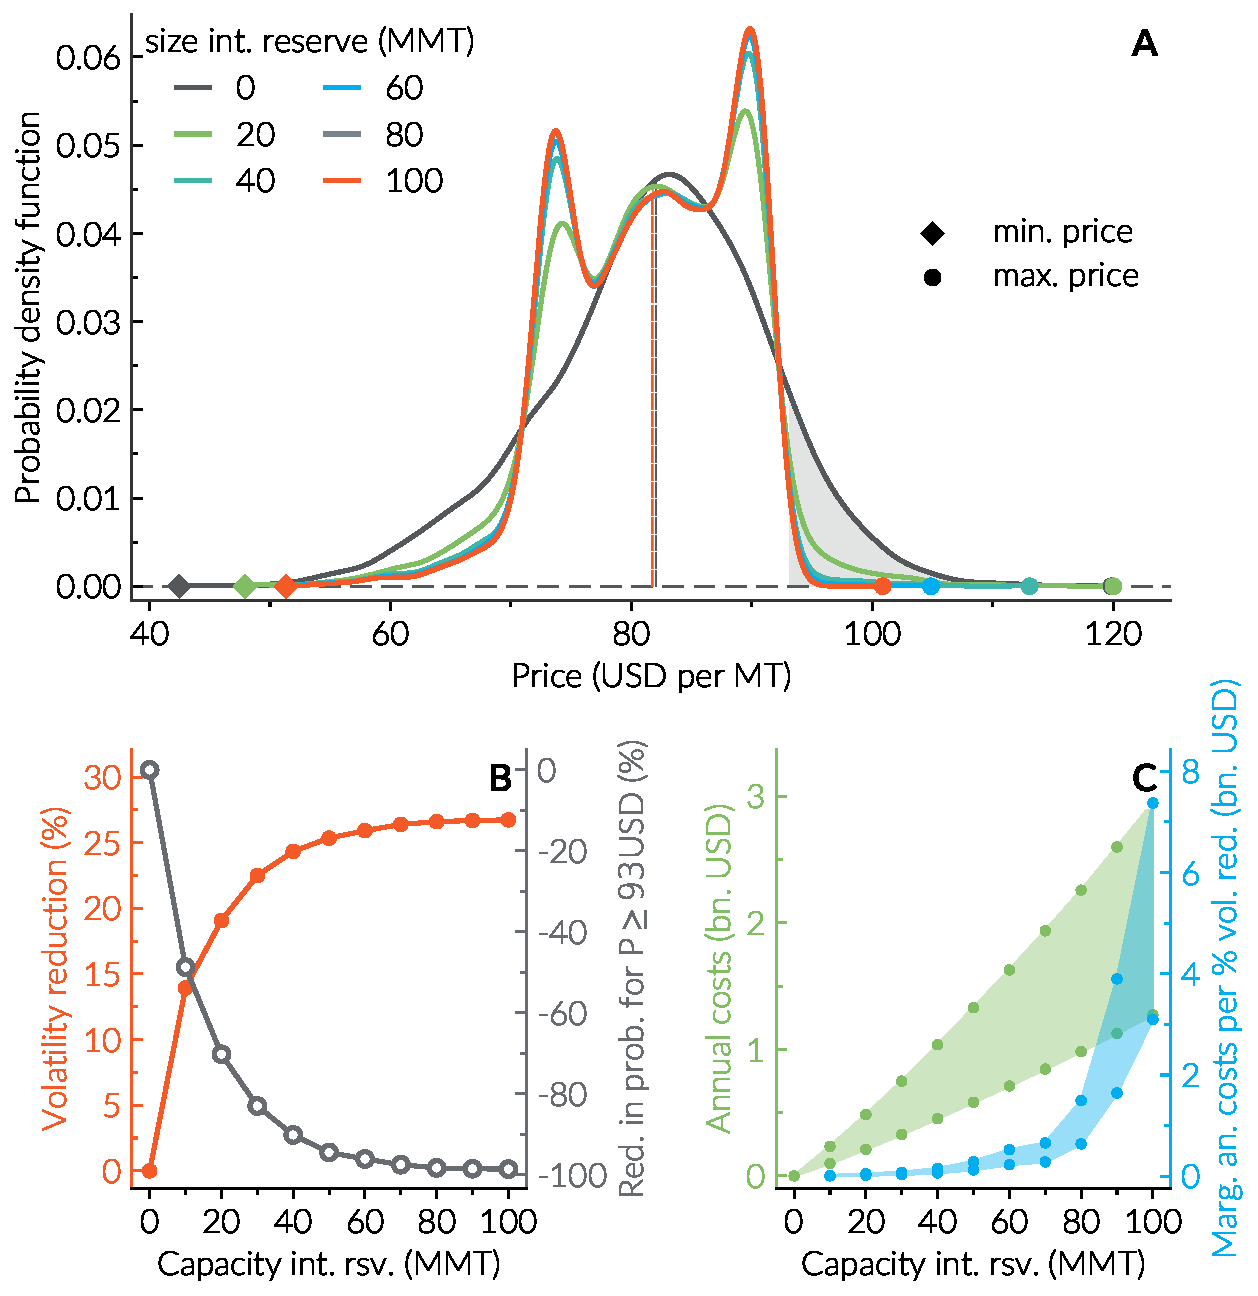
\includegraphics[width=.8\textwidth]{plots/arti_ts_2010_15/pdf_and_costs2grid.pdf}
\caption{Reduction of price volatility and costs for different sizes of the international reserve.  \textbf{A}: Probability density function. Diamonds and filled dots denote minima and maxima of price time series, respectively. Vertical dashed lines indicate the means of the price distributions. \textbf{B}: Volatility reduction in percent (orange dots, left y-axis) and reduction of the probability of occurrence for prices $P\geq 93$\USD, i.e., above the 90\textsuperscript{th} percentile of the price distribution for the full historical scenario (w/o reserve); see gray shaded area in A. \textbf{C}: Costs (green, left y-axis) and marginal costs for volatility reduction (blue, right y-axis) in dependence of reserve size. The price band has a width of 18\USD.}
  \label{fig:Fig3}
\end{figure}

\clearpage
\appendix
%\afterpage{\clearpage}
%\onecolumn
\setcounter{figure}{0}
\setcounter{table}{0}
\renewcommand{\thetable}{S\arabic{table}}
\renewcommand{\thefigure}{S\arabic{figure}}

\section*{Supplementary Material (SI)}
\label{sec:SI}
The SI is structured as follows: first, we discuss the data used in our study and derive the regions' crop calendars in Sec.~\ref{si:MM}. Then, we give a comprehensive model description in Sec.~\ref{si:modDet}, before eventually providing details on the different scenarios discussed in the main text in Sec.~\ref{si:scen}.  

\section{Materials and Methods}
\label{si:MM}
Regional consumption, annual production, and ending stock data are derived from the Production,
Supply, and Distribution database of USDA's Foreign Agricultural Service
(USDA-PSD)\footnote{\url{https://apps.fas.usda.gov/psdonline}, accessed June, 2017.}.  For the
simulations presented in this study, we group the countries contained in the USDA-PSD database into
five agricultural regions. Four of them, EUR, FSU, NAF, and CPA, are the world's main wheat
producing regions, and the rest of the countries is lumped together in the ROW region. Country names
and the number of countries accounted for in the database have been changing over time.
Table.~\ref{tab:conGroup} shows the assignment of all (present as well as former) countries and
groups of countries (e.g., EUR-15) included in the database for the international trade years 1980
to 2016 to the five agricultural regions of this study.
\begin{table}[htbp]
  \caption{Grouping of countries into the five agricultural regions: European Union (EUR), Former Soviet Union (FSU), North Atlantic Free Trade countries (NAF), Centrally Planned Asia (CPA ), and rest of the world (ROW). Country names are stated as given in the USDA-PSD online database.}
  \label{tab:conGroup}
  \centering
    \begin{tabularx}{\textwidth}{lX}
      Region & Country\\
      \toprule
      \multirow{2}{*}{CPA} & China, Hong Kong, Democratic People's Republic of Korea, Mongolia, Singapore, Taiwan, Viet Nam\\
      \midrule
      \multirow{3}{*}{FSU} & Armenia, Azerbaijan, Belarus, Georgia, Kazakhstan, Kyrgyzstan, Republic of Moldova, Russian Federation, Tajikistan, Turkmenistan, Union of Soviet Socialist Republics (USSR), Ukraine, Uzbekistan\\
      \midrule
      \multirow{4}{*}{EUR} & Albania, Bosnia and Herzegovina, Bulgaria, Croatia, Cyprus, Czechia, EU-15, Estonia, European Union, Former Czechoslovakia, Hungary, Latvia, Lithuania, Republic of Macedonia, Malta, Norway, Poland, Romania,
        Serbia, Serbia and Montenegro, Slovakia, Slovenia, Switzerland, Socialist Federal Republic of Yugoslavia \\
      \midrule
            NAF & Canada, Mexico, United States\\
      \midrule
      \multirow{14}{*}{ROW}
             & Afghanistan, Algeria, Angola, Argentina, Australia, Bahrain, Bangladesh, Barbados, Benin, Bhutan, Plurinational State of Bolivia, Brazil, Burkina Faso, Cameroon, Chad, Chile, Colombia, Congo, The Democratic Republic of the Congo, Costa Rica, Cuba, Cote d'Ivoire, Dominican Republic, Ecuador, Egypt, El Salvador, Eritrea, Ethiopia, Fiji, Gabon, Ghana, Guatemala, Guinea, Guyana, Haiti, Honduras, India, Indonesia, Islamic Republic of Iran, Iraq, Israel, Jamaica, Japan, Jordan, Kenya, Republic of Korea, Kuwait, Lebanon, Lesotho, Liberia, Libya, Madagascar, Malawi, Malaysia, Mali, Mauritania, Mauritius, Morocco, Mozambique, Myanmar, Namibia, Nepal, New Zealand, Nicaragua, Niger, Nigeria, Oman, Pakistan, Panama, Papua New Guinea, Paraguay, Peru, Philippines, Rwanda, Saudi Arabia, Senegal, Sierra Leone, Somalia, South Africa, Sri Lanka, Sudan, Syrian Arab Republic, United Republic of Tanzania, Thailand, Togo, Trinidad and Tobago, Tunisia, Turkey, Uganda, United Arab Emirates, Uruguay, Bolivarian Republic of Venezuela, Yemen, Yemen (Aden), Yemen (Sanaa), Zambia, Zimbabwe\\
      \bottomrule
    \end{tabularx}
    %\addtabletext{MENA\ldots}
  \end{table}
  Nominal WM prices for US hard red winter wheat are taken from the Commodity Markets online
  database of the World Bank\footnote{http://www.worldbank.org/en/research/commodity-markets,
    accessed June, 2017.}, and real prices are obtained by deflating with the US All Urban Consumers
  price index (June 1983 = 100) provided by the US Bureau of Labor
  Statistics\footnote{https://www.bls.gov, accessed June, 2017.}. Further, the regional crop
  calenders, i.e., the percentage of production harvested in each time step is calculated by
  combining data on the harvesting season for winter wheat from \cite{SAC10} (interpolated dataset
  with 5\minute~by~5\minute~resolution) with harvested areas and yields for the year 2000
  taken from a global gridded, observational dataset \cite{MON08} (same resolution) obtained from
  remote sensing. For each grid cell, we assume that there is one harvest per year, which is normal
  distributed. In order to obtain the regional harvest distributions (Fig.~\ref{fig:crop_cal}), this
  distribution is weighted by the cell's production, and aggregated over each agricultural
  region. The model is implemented in python; the program code is available upon request.
\begin{figure}[htbp]
  \centering
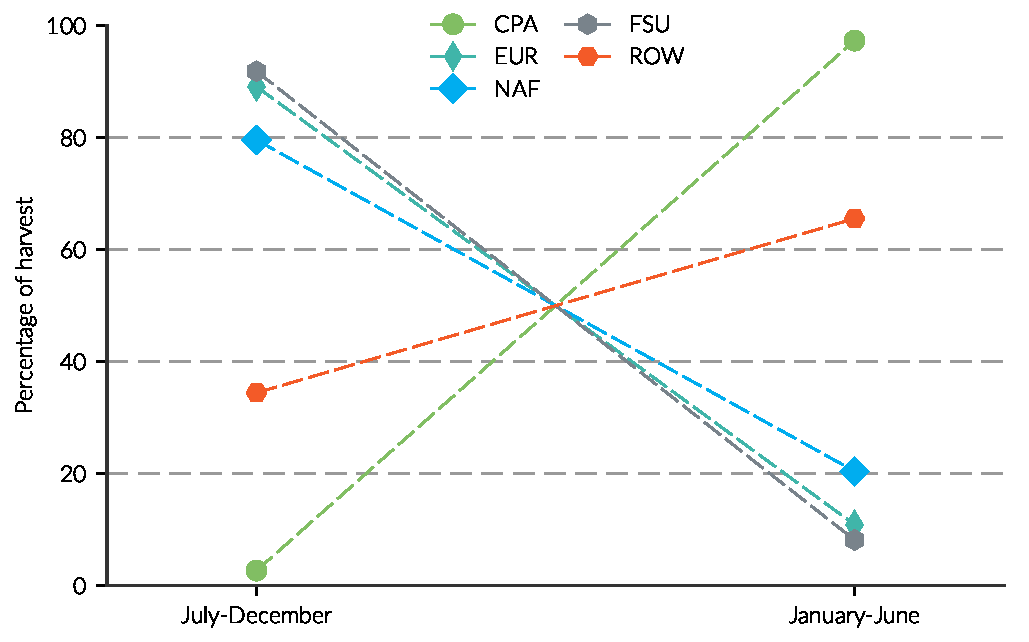
\includegraphics[width=.8\textwidth]{plots/crop_calendar/crop_cal_gridded}
\caption{Crop calendar for the five agricultural regions: European Union (EUR), Former Soviet Union (FSU), North Atlantic Free Trade countries (NAF), Centrally Planned Asia (CPA), rest of the world (ROW). The international trade year for wheat spans from July to June, in accordance with the USDA-PSD online database.}
  \label{fig:crop_cal}
\end{figure}

\section{Modeling details}
\label{si:modDet}
The subsequent section provide a comprehensive model description. First, we discuss the rationales
of the various economic agents in Sec.~\ref{si:econAgents}, before describing their interaction on
the WM in Sec.~\ref{si:market_dyn}. Then, we provide details on the implementation of stockkeeping
policies short-term market interventions in Sec.~\ref{si:trad_pol}, and, eventually, discuss the
initial conditions in Sec.~\ref{si:iniCond}. A summary of the exogeneous parameters used in the
simulations is provided in Tab.~\ref{tab:params}.
\begin{table}[htbp]
  \caption{Exogeneous parameters of the model used in the simulations if not indicated otherwise. $\langle\cdot\rangle_a$ denotes the temporal average of the last $a$ years. Regional parameters are identical for all regions if not states otherwise.}
  \label{tab:params}
  \centering
    \begin{tabular}{lll}
      Meaning & Symbol & Value \\
      \toprule
      No. of timesteps per year & $N$ & $2$\\
      Storage costs & $k_r$ & $20\USD/\Mt/\annum$\\
      Loss rate & $\rl_r$ & $3.5\%/\annum$\\
      Interest rate & $\gamma$ & $2.5\%/\annum$\\
      Maximum consumer price & $\Pmax_r$ & $435\USD$\\
      Price elasticity & $\ec$ & $0.4$\\
%      Demand elasticity & $\dce_r$ & in sim. demand set to hist. data\\
      Reference price & $\Pref$ & $90\USD$\\
      \midrule
      Capacity of strategical storage & $\Ismaxr$ & see Sec.~\ref{si:trad_pol}\\
      Strength of export restriction & $\erd_r$ & see Sec.~\ref{si:trad_pol}\\
      \midrule
      Center price of price band & -- & $\av{P}{15}$\\
      \bottomrule
    \end{tabular}
  \end{table}

\subsection{Economic agents}
\label{si:econAgents}
As described in the main text, the agricultural economic activities in each region $r\in R$
of the set of regions $R$ are described by three agents: a commercial storage holder, a
strategic storage holder, and a domestic consumer. Their rationales are detailed in the subsequent
paragraphs.

\paragraph*{Commercial storage holder}
We model the commercial storage holder of a region $r$ as a risk-neutral
bounded-rational agent. At each timestep $t$, the agent receives an amount of grain $h_r^t$
harvested in the region and then plans its WM supplies
$\bs y_r^t\equiv(y_r^0,\ldots,y_r^{N-1})^{\bot}$ by maximizing expected profit over the forecasting
period split into $N$ timesteps. Expected profit is calculated from the difference between expected
revenues and warehousing costs in this period reading
\begin{equation}
  \label{eq:exp_profit} \hPi_r(\bs y_r)\equiv
\sum_{n=0}^{N-1}\frac{\hP_r^n(y_r^n)\, y_r^n}{(1+\gamma)^n} -k_r\sum_{n=0}^{N-1}
n\, y_r^n.
\end{equation}
Here, $\hP_r^n$, $\gamma$, and $k_r$ denote the agent's expectation on the WM price at time $t+n$,
the interest rate, and the storage costs per timestep, respectively. The expected profit depends on
the agent's expectation on future WM prices. To form these expectations, the agent estimates (i) its
own impact on WM price, (ii) its own harvest in the next year, (iii) the WM supplies of its
competitors during this period, and (iv) WM demand. Here, we assume that all regional agents have
access to the same global supply and demand forecasts provided for instance by the Food and
Agricultural Agency (FAO) of the UN or by the quarterly Supply and Demand forecasts of the United
States Department of Agriculture (USDA) providing them with a foresight horizon of one year.

Having no precise knowledge on future WM supplies of its competitors and future demand side
stockholding policies, the agent assumes a simple iso-elastic dependence of WM price on WM supply
reading
\begin{equation}
  \label{eq:exp_WM_price}
P_r^n(y_r^n)\equiv \Pref \left(\frac{\hS_r^{R,n}+y_r^n}{\hD_n} \right)^{\frac{1}{\ec}},
\end{equation}
where $\Pref$, $\hS_r^{R,n}$, $\hD_n$, and $\ec$ denote a reference price, the agent's expectation
on the WM supply of its competitors, expected WM demand, and the price elasticity of WM supply,
respectively. The agent calculates $\hS_r^{R,n}$ by taking the supply forecast of the international
agency $\hS^n$ and subtracting its own expected contribution $\hs_r^n \hS^n$ yielding
\begin{equation}
  \label{eq:SROW}
  \hS^{R,n}_r \equiv (1- \hs_r^n) \hS^n.
\end{equation}
Here, we assume that the agent estimates its share $\hs_r^n$ on future WM supply by averaging over
its shares in the last 2 years. The global supply and demand forecasts, $\hS_n$ and $\hD_n$, are
derived from USDA production and domestic consumption data smoothed with a Savitzky-Golay filter
with a window size of 31 years (see Fig.~\ref{fig:supProd_and_cons}(global)).
\begin{figure}[htbp]
  \centering 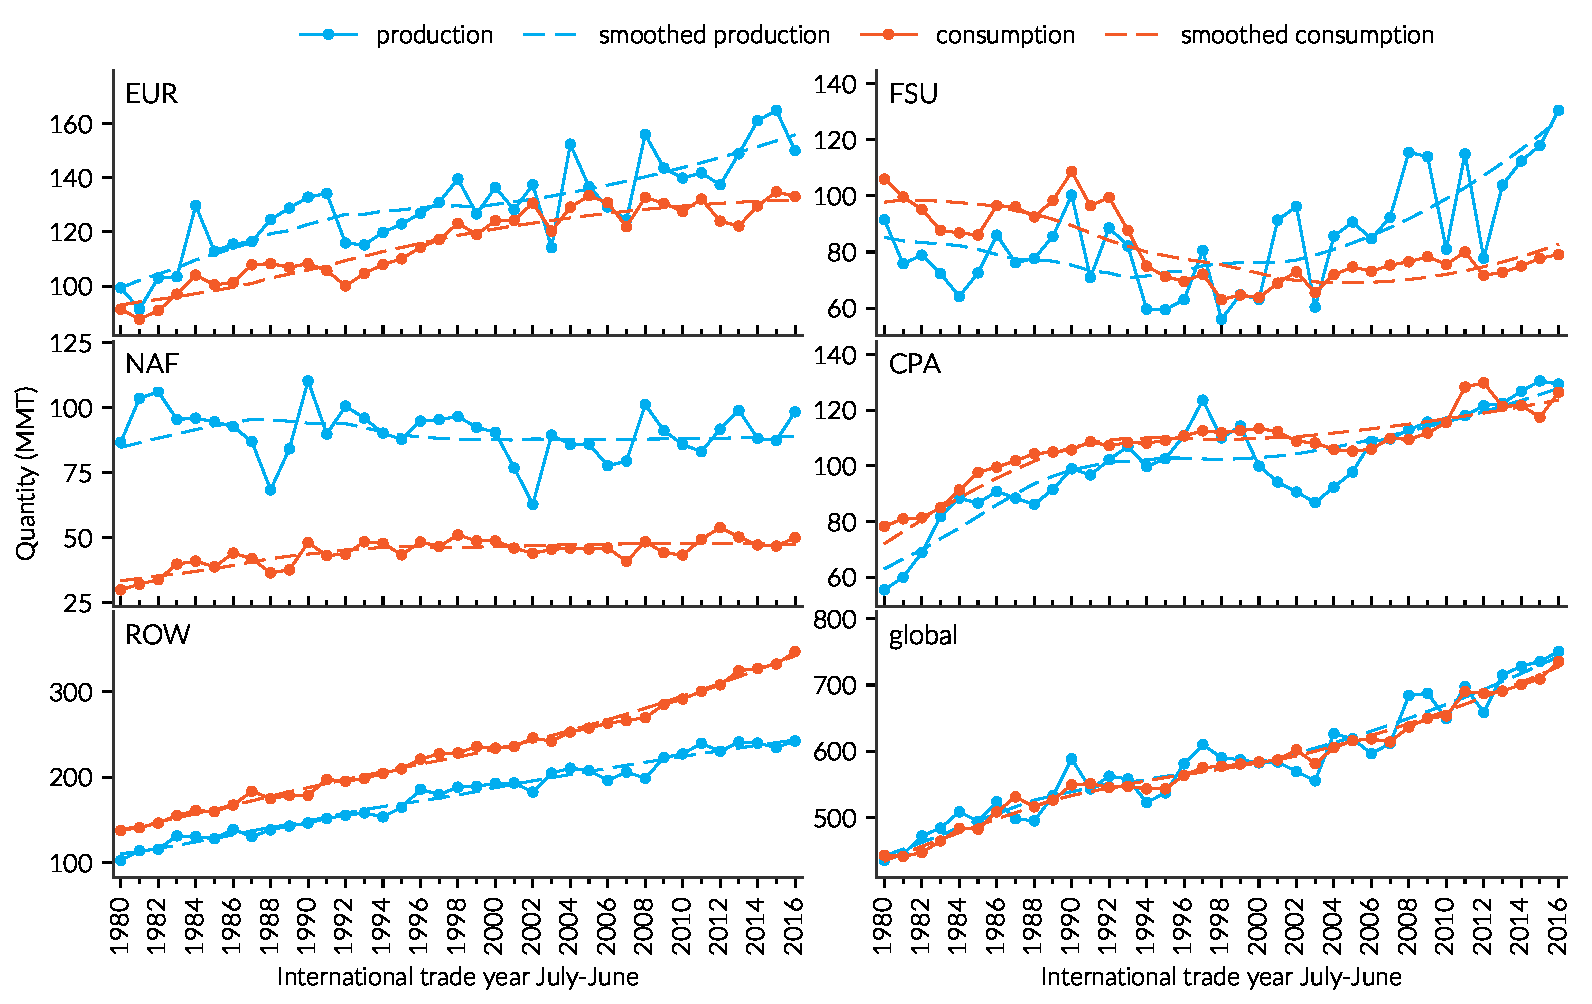
\includegraphics[width=.8\textwidth]{plots/USDA_supply_and_demand/prod_cons_1980_2016.pdf}
  \caption{Historical production and domestic consumption data as reported by USDA for the five main
    agricultural regions: European Union (EUR), Former Soviet Union (FSU), North Atlantic Free Trade
    Agreement countries (NAF), Centrally planned Asia (CPA), the rest of the world (ROW) as well
    as globally (global). Dashed lines indicated smoothed data used for the global supply and demand
    forecasts. The international trade year spans from July to June.}
  \label{fig:supProd_and_cons}
\end{figure}

Finally, the commercial storage holder obtains the optimal distribution of WM supplies $\yropt$ by
maximizing $\hPi_r$ over the forecast period under the constraints that (i) all supplies have to be
non-negative, (ii) they must not exceed its expected storage content, and (iii) export restrictions
may temporally limit the amount of grain it can sell on the WM yielding the following constraint
optimization problem
\begin{subequations}
\label{eq:yopt}
\begin{align}
  &\yropt \equiv \underset{\bs y_r}{\argmax}\left[\hPi_r(\bs y_r)\right],\text{ subject to}\\
  &y_r^n \geq 0\,\, \forall n\,\wedge\, \bs L\cdot \bs y_r \leq (1-\erd_r)\left[I_r\mathbb{I} + \bs L \cdot\bs \hh_r\right]\label{subeq:capac_constraint}.
\end{align}
\end{subequations}
Here, $\bs L$ denotes a lower triangular matrix of ones, `$\cdot$' is the scalar product, and
$\erd_r\in[0,1]$ is the share of the agent's expected storage content that it cannot sell on the WM
in case of a regional export restriction. Further, $\mathbb{I}$, $I_r$ denote the identity vector,
and the agent's storage content, respectively. For simplicity, we assume that the agent's estimates
on its own upcoming harvests $\bs \hh_r$ within the forecast period are perfect.

\paragraph*{Strategic storage holder}
The strategic storage holder aims at providing food security for the region's domestic
consumption. In contrast to the commercial storage holder, the strategic storage holder aims to
assure a certain inventory level instead of maximizing profit. We assume that its demand decreases
linearly with price (see also \cite{SCH17} for a detailed discussion)
\begin{equation}
  \label{eq:D_r}
  D_r(P)\equiv\max\left[\Dmax_r\Big(1 - \frac{P}{\Pmax_r}\Big),0\right],
\end{equation}
where $\Dmax_r\equiv \Ismaxr - I_r^{s,t-1}$ is the available storage space given by the difference
between total storage capacity $\Ismaxr$, an exogeneous measure for the region's target inventory
level, and $I_r^{s,t-1}$, the inventory carry over from the last time step. Further, $\Pmax_r$
denotes the maximum price up to which the agent is willing to purchase a non-zero amount.

\paragraph*{Domestic consumer}
The third agent type represents the region's domestic consumption, which is assumed to depend
iso-elastically upon WM price. We assume that domestic consumers do not directly purchase grain from
the WM, but refer to the region's strategic storage. Consequently, this agent's consumption is
limited by the content of the strategic storage, $I_r^{s,t-1}+D_r(P)$. Unless stated otherwise,
annual regional consumption is fixed to the values reported by USDA. However, for some simulations,
we assume an iso-elastically dependence of regional consumption upon WM price
\begin{equation}
  \label{eq:C_r}
 C_r(P)\equiv \min\left[\Cref_r\left(\frac{P}{\Pref_r} \right)^{\dce_r},I_r^{s,t-1}+D_r(P)\right],
\end{equation}
where $\Cref_r\equiv\Cref_r(\Pref_r)$ denotes the reference level of domestic consumption estimated
from past values of domestic consumption, and $\dce_r$ denotes the region's demand elasticity. The
latter may vary among regions, which accounts for their different dependencies upon the modeled
crop.

\subsection{Market dynamics}
\label{si:market_dyn}
We assume that the market clears in each timestep, and the equilibrium price $\Peq$ is determined by
equating WM supply $S\equiv \sum_{r\in R} \yropt$ and WM demand $D(P)\equiv \sum_{r\in R}D_r(P)$,
i.e., we obtain $\Peq$ by solving $S=D(\Peq)$ for $\Peq$. Next, the inventories of commercial and
strategic storage holders are updated according to the rules
\begin{align}
  \label{eq:stor_update}
  I_r &= (1-\rl_r)\,I_r^{t-1} -y_r + h_r, \\
  \Isr &= (1-\rl_r)\,I_r^{s,t-1} + D_r(\Peq)-C_r(\Peq),
\end{align}
where $\rl_r$ is the loss rate for storing grain, $I_r^{t-1}$ and $I_r^{s,t-1}$ denote the
carry-over stocks of region $r$'s commercial and strategic storage holders, respectively, and $h_r$
denotes the region's harvest in the present timestep. The loss rates $\rl_r$ for crop spoilage are
identical for all regions as well as for the international reserve. They are estimated from best fit
of the ending stocks for the scenario accounting only for regional production and consumption
variabilities (see Sec.~\ref{si:scen} for details).

% \paragraph*{Trade policies}
% We consider two types of regional trade policies: changes in strategic
% stockholding policies and export restrictions. A stockholding policy in region
% $r$ is modeled by varying $\Ismaxr$ (cf.~Eq.~(\ref{eq:D_r})), which is a proxy
% for the region's target inventory level. Further, we assume that other important
%   consumer side policy measures such as import subsidies can be also represented
%   by changes in $\Ismaxr$.. These policies determine the stocks-to-use (stu)
% ratio, which is perceived as the optimal tradeoff between food security in times
% of scarcity and costs in normal times. Consequently, reported stu-ratios,
% calculated from the ratio of ending stocks and domestic consumption, differ
% significantly among regions, and they change over time (see
% Fig.~\ref{fig:stuRatios} in SI). For instance, the abrupt decline of ending
% stocks in the NAF region between $1986$ and $1988$ marks the transition from
% governmentally managed stocks to a market-oriented stockholding scheme
% \cite{WES99} (see ending stocks and stu-ratio for NAF region in
% Fig.~\ref{fig:Fig2} and Fig.~\ref{fig:stuRatios} in SI, respectively). We use
% these regional changes in stu-ratios as proxies for regional changes in the
% demand for strategic stockholding expressed by $\Ismaxr$ in the model
% (cf.~Eq.~(\ref{eq:D_r})).

% Further, major reported national export restrictions are implemented by non-zero
% values of $\erd_r$ (cf.~Eq.~(\ref{subeq:capac_constraint})). Since export
% restrictions are short-term policy measures in times of crises, we assume that
% agents cannot foresee the onset of export restrictions nor their revocation. The
% commercial storage holder of the region imposing the export restriction
% therefore assumes that, once imposed, the restriction will remain in place for
% the whole foresight period.

% Since it is not possible to derive the absolute values of both $\Ismaxr$ and
% $\erd_c$ directly from the trade data, these parameters are determined by best
% fit of simulated prices and regional ending stocks with the reported
% ones. Details on the implementation of policies are discussed in
% Sec.~\ref{si:trad_pol} of the SI and Tab.~\ref{tab:tradPol} lists the policies
% that we account for, their timing, and reporting sources.

% \paragraph*{International reserve}
% \label{sec:int_reserve}
% The price stabilization reserve is a measure designed to reduce price volatility
% by stabilizing prices within a certain price band $\Peq\in[\Pfl,\Pceil]$
% centered around a center price $\Pc$, representing market fundamentals. The
% price band is limited from below by a floor price $\Pfl$ and from above by a
% ceiling price $\Pceil$. If $\Peq$ drops below $\Pfl$, the reserve is filled by
% purchases from the WM until $\Peq$ increases above $\Pfl$ or the reserve is
% filled to its capacity. If $\Peq$ exceeds $\Pceil$, grain is released from the
% reserve onto the market until either $\Peq$ drops below $\Pceil$ or the reserve
% is depleted.


\subsection{Policies}
\label{si:trad_pol}
In this section, we discuss the calibration of the model with respect to the capacities of the
strategic inventories $\lbrace\Ismaxr\rbrace_r$, which are proxies for the regions' target demand
for strategic stockkeeping, and the factors $\lbrace\erd_c\rbrace_r$, which are measures for the
strengths of regional export restrictions. As discussed in the main text, we use reported changes of
a region $r$'s annual stu-ratio as a proxy for changes in $\Ismax_r$.  Further, we assume that other
measures for the protection of domestic consumers as for instance import subsidies can be also
represented by changes in the $\lbrace \Ismax_r \rbrace_r$.

To obtain $\Ismax_r$ for region $r$'s strategic storage holder, from the time series of the region's
reported stu-ratio $\rstu_r$, we first determine intervals in which this ratio does not vary
significantly. In these intervals, we then set $\Ismaxr$ to a multiple $m_r$ of the mean stu-ratio
in this interval $\avrstu_r$ multiplied by the region's mean domestic consumption in the last three
years and its mean expected consumption within the foresight period $\langle C_r\rangle_{3+1}$,
i.e., $\Ismaxr$ reads
\begin{equation}
  \label{eq:Ismaxr}
  \Ismaxr \equiv m_r\avrstu_r \langle C_r\rangle_{3+1}.
\end{equation}
\begin{figure}[htbp]
  \centering
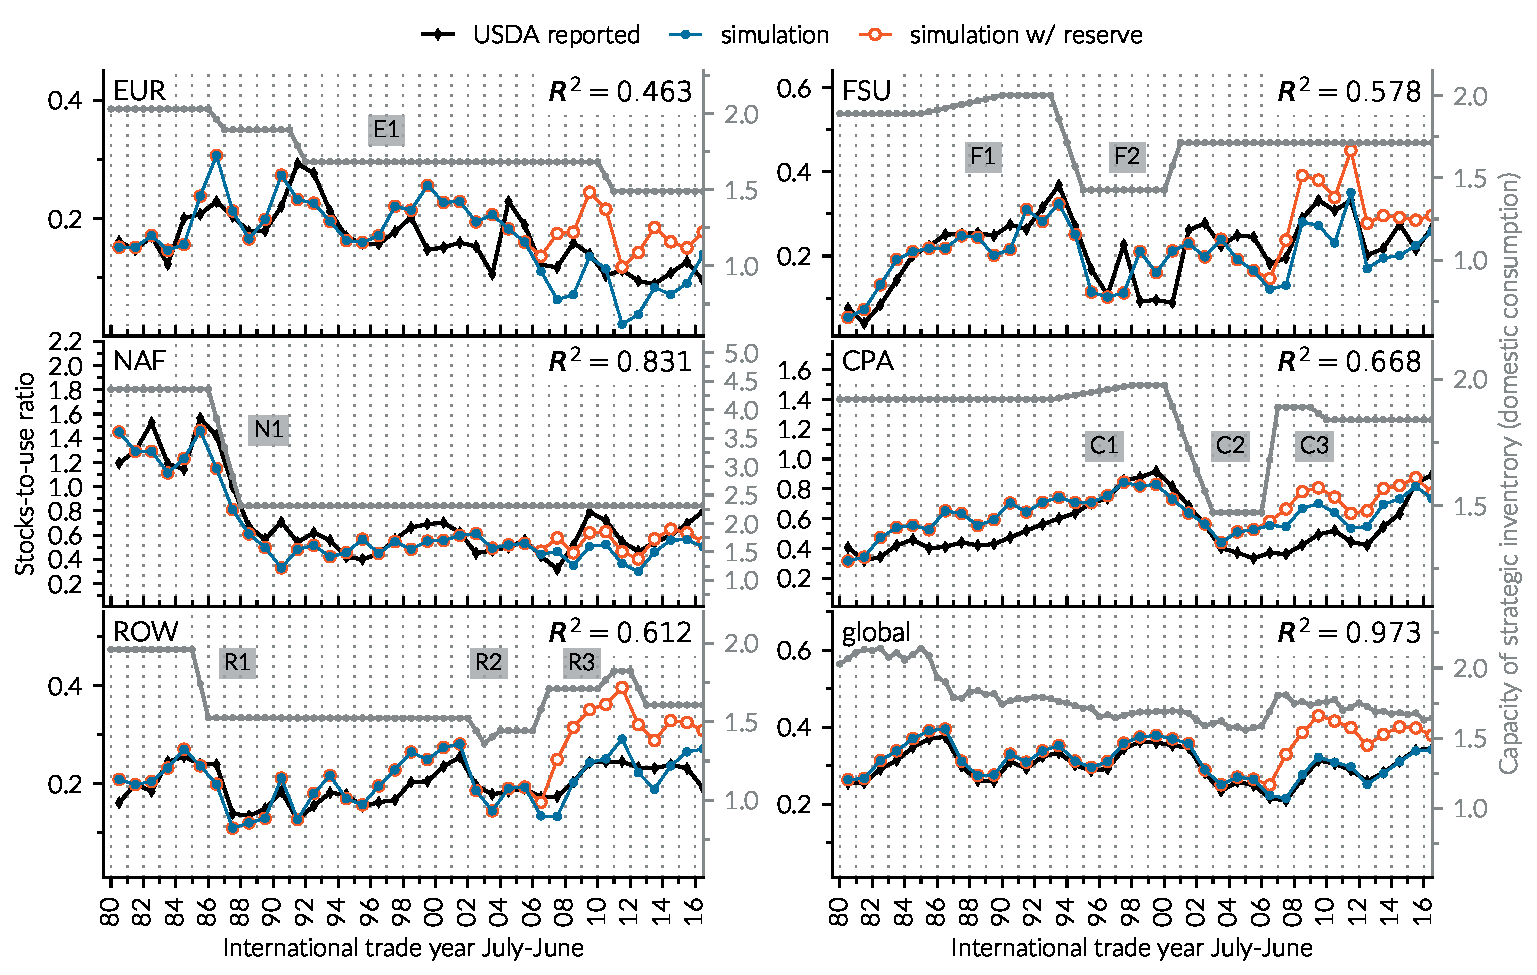
\includegraphics[width=.8\textwidth]{plots/full/Stocks-to-use_ratio_1980_2017}
\caption{Stocks-to-use (stu) ratios for the five economic regions: European Union (EUR), Former
  Soviet Union (FSU), North Atlantic Free Trade countries (NAF), Centrally Planned Asia (CPA), rest
  of the world (ROW), as well as globally (global). Black diamonds, blue dots, and open orange
  circles, indicate ending stocks as reported by USDA, for the historical scenario without and with
  international reserve, respectively. Squared Pearson correlation coefficients $R^2$ denote the
  correlation between reported stu-ratios and the simulation without reserve. Small gray dots
  ($\secnd$ y-axes) denote the capacity of the regions's strategic reserves in multiples of domestic
  consumptions (cf.~ Eq.~(\ref{eq:Ismaxr})). Capacity changes result from the policies (labels in
  gray rectangles) listed in Tab.~\ref{tab:tradPol}. Parameters are as in Tab.~\ref{tab:params}.}
  \label{fig:stuRatios}
\end{figure}
Policy changes are represented by linearly connecting the intervals of constant $\avrstu_r$. The
absolute level of $\Ismax_r$, i.e., the multiple $m_r$, is determined by the best fit of modeled
prices and regional ending stocks with their observed counterparts. Fig.~\ref{fig:stuRatios} depicts
regional observed annual stu-ratios (black diamonds) as well as the simulated stu-ratios for the
scenarios without (blue dots) and with (open orange circles) international reserve; the second
y-axes depict the products of the multiples $m_r$ and fitted stu-ratios $\rstu_r$. Further, we
have verified that all policies accounted for in our simulations are reported in the literature. In
Fig.~\ref{fig:stuRatios}, these policies are labeled by gray rectangles with one-letter codes of the
economic regions issuing the policy followed by ascending numbers. Descriptions of policies, their
timing, and reporting sources are summarized in Tab.~\ref{tab:tradPol}.

\paragraph*{Export restriction}
Export restrictions in a region $r$ are modeled by non-zero values of $\erd_r$. We first identified
the major export restrictions by a literature research. The specific value that $\erd_r$ assumes
when a export restriction is in place is determined by the best fit of simulated prices and ending
stocks with their reported counterparts. All export restrictions accounted for in the simulations,
their timing, and the reporting literature sources are listed in Tab.~\ref{tab:tradPol}.
\begin{table}[ht]
  \caption{Reported policies taken into account in the simulations to reproduce historical prices and ending stocks. The lower part of the table describes export restrictions. The parameter values of $\erd_R$ (cf. Eq.~(\ref{subeq:capac_constraint})) used in the simulations are given in rounded brackets.}
  \label{tab:tradPol}
  \centering
    \begin{tabularx}{\textwidth}{llX}
      Event label & Time period & Description \\
      \toprule
      \multirow{2}{*}{E1} & \multirow{2}{*}{early  90s -- mid 00s}
                          & Gradual reduction of governmental stocks in EU to comply with Uruguay Round of WTO \cite{WB12}.\\
      \midrule
      \multirow{1}{*}{F1} & \multirow{1}{*}{80s} & Increase in strategical stocks in USSR \cite{AND08}.\\
      \addlinespace
      \multirow{3}{*}{F2} & \multirow{3}{*}{early 90s -- early 00s} & Decline and subsequent recovery of stocks due to restructuring of agricultural production and trade after breakdown of USSR \cite{AND08, LIE13}.\\
      \midrule
      \multirow{2}{*}{N1} & \multirow{2}{*}{1985} & Reduction of governmental stocks in US during transition to market-oriented stockholding policies \cite{WES99}.\\
      \midrule
      \multirow{2}{*}{C1} & \multirow{2}{*}{90s}& Accumulation of governmental stocks due to strong producer support \cite{FAO99,HSU01}.\\
      \addlinespace
      \multirow{2}{*}{C2} & \multirow{2}{*}{1999 -- 2004} & Decrease of stocks due to grain marketing and reserve reform in the course of China's WTO accession \cite{DAW09,HSU01}.\\
      \addlinespace
      \multirow{1}{*}{C3} & \multirow{1}{*}{2008 \& 2011} & Unusual purchases by China to restock inventories \cite{TRO11}.\\
      \midrule
      \multirow{2}{*}{R1} & \multirow{2}{*}{90s} & Reduction of public stockholding in OECD countries to comply with Uruguay Round of WTO \cite{WB12}.\\
      \addlinespace
      \multirow{2}{*}{R2} & \multirow{2}{*}{2003 -- 2004} & Unusual high exports of India and Brazil due to record stock levels\footnote{USDA's PSD online database \url{https://apps.fas.usda.gov/psdonline}, accessed June 2017}.\\
      \addlinespace
      \multirow{2}{*}{R3}
            & \multirow{1}{*}{2008} & Unusual purchases India, Iran, Mexico, MENA \cite{HEA08}.\\
            & \multirow{1}{*}{2011} & Build-up of food security stocks in MENA \cite{TRO11}.\\
      \midrule\midrule
            & \multirow{1}{*}{10/2006 -- 5/2007}  & Export quota Ukraine \cite{SHA11} ($\erd_{\FSU}=0.1$).\\
            & \multirow{1}{*}{6/2007 -- 5/2010}  & Export (quasi) ban Ukraine \cite{SHA11} ($\erd_{\FSU}=0.2$).\\
            & \multirow{1}{*}{8/2010 -- 4/2011}  & Export quota Ukraine \cite{SHA11} ($\erd_{\FSU}=0.15$).\\
       & \multirow{1}{*}{4/2008 -- 10/2008} & Export ban Kazakhstan \cite{SHA11} ($\erd_{\FSU}=0.2$).\\
       & \multirow{1}{*}{8/2010 -- 10/2011}  & Export ban Russia \cite{TRO11,GrainChain12} ($\erd_{\FSU}=0.15$).\\
      \bottomrule
    \end{tabularx}
 \end{table}
% \afterpage{\clearpage}

\subsection{Initial conditions}
\label{si:iniCond}
For calibration, it is convenient to run the model from a steady state close to the state given by
the annual production and consumption data of the simulation's start year. Note that, in general,
global annual production and consumption do not match, and the simulation's start year therefore
usually does not constitute a steady state of the dynamical system.

We construct the initial steady state by taking the regional productions of the start year, and
modifying regional consumption such that global consumption equals global production. For that, we
first determine the share of global consumption that each region has in the start year. Then,
regional consumptions are determined by multiplying these shares with the global production of the
start year.

\paragraph{Inventory of competitive storage holder}
We assume that in the initial steady state, the commercial storage holder of a region does not carry
over any inventory from one local agricultural year to the next, i.e, for biannual time steps, the
agent sells in average one half of its annual harvest in each time step on the WM. Note that, if the
local agricultural year differs from the international trade year (July to June), the agent can
nevertheless have finite ending stocks at the end of the latter, i.e, in June. Thus, the competitive
storage holders of EUR, FSU, and NAF, which have their harvest maximums in the first semester the
international trade year have zero ending stocks. In contrast to the competitive storage holders of
CPA and ROW, which have their harvest maximums in the second semester of the international trade
year and therefore have finite ending stocks. Summing up, ending stocks of the strategical storage
holders in the steady state read
\begin{equation}
  \label{eq:ES_strat_stor}
  I_r^{\star,2}\equiv\begin{cases}
    0, & \text{for }r\in[\EUR, \FSU, \NAF],\\
    \hrstar(\nu_{h,r}^{\star,2}-\frac{1}{2}), & \text{for }r\in[\CPA,\ROW],
  \end{cases}
\end{equation}
where $\hrstar$ and $\nu_{h,r}^{\star,2}$ denote region $r$'s harvest in the start year of the
simulation and the fraction harvested in the second semester of the international trade year,
respectively.

\paragraph{Inventory of strategical storage holder}
We assume that in the initial steady state the strategical storage holder's inventory content
remains constant, i.e., in each time step, the amount of grain purchased on the WM by region $r$'s
strategical storage holder equals the domestic consumption in this region. Thus, by taking the
ending stocks reported for the simulation's start year $I_r^{\sigma,\star,2}$ and subtracting the
ending stock of $r$'s competitive storage holder $I_r^{\star,2}$, we may obtain the ending stocks of
$r$'s strategical storage holder as
\begin{equation}
  \label{eq:ES_strat}
 I^{s,\star,2}_r\equiv I_r^{\sigma,\star,2} - I_r^{\star,2}.
\end{equation}
Next, we calculate the inventory size needed to ensure that $r$'s strategical storage holder
purchases on the WM equal $r$'s consumption $\starC_r\equiv \starC_r(\starP)$ in the steady
state. Here, $\starP$ denotes the WM price in the steady state, which is set to the WM price in the
first semester of the simulation's start year. For that, we equate $\starC_r$ to the demand of $r$'s
strategic storage holders, which reads according to Eq.~(\ref{eq:D_r})
\begin{equation}
  \label{eq:starCr}
  \starC_r = (\starIsmax_r - I_r^{s,\star,2}) \left(1-\frac{\starP}{\starPmax_r} \right).
\end{equation}
Solving the above equation for $\starIsmax_r$ then yields
\begin{equation}
  \label{eq:IrmaxIni}
  \starIsmax_r \equiv \frac{\starC_r}{1 - \starP/\Pmax_r}  + I_r^{s,\star,2}.
\end{equation}
Eventually, we set the spoilage rate equal to zero ($r^l=0$) in the steady state.

% \section{Country grouping}
% \label{si:country_grouping}
% For the simulations presented in this study, we group the countries contained in
% the USDA-PSD database into five agricultural regions. Four of them, EUR, FSU,
% NAF, CPA, are the main wheat producing regions, and the rest of the countries is
% lumped together in the ROW region. Country names and the number of
% countries accounted for in the database have been changing over time.
% Table.~\ref{tab:conGroup} shows the assignment of all (present as well as
% former) countries and group of countries (e.g., EUR-15) included in the database
% for the years $1980$ to $2016$ to the five agricultural regions of this study.
% \begin{table}[htbp]
%   \caption{Grouping of countries into the five agricultural regions: EUR (Europe 28), FSU (Former Soviet Union), NAF (North Atlantic Free Trade Agreement countries), CPA (Centrally Planned Asia), ROW (rest of the world). Country names are stated as given in the USDA-PSD online database.}
%   \label{tab:conGroup}
%   \centering
%     \begin{tabularx}{\textwidth}{lX}
%       Region & Country\\
%       \toprule
%       \multirow{2}{*}{CPA} & China, Hong Kong, Democratic People's Republic of Korea, Mongolia, Singapore, Taiwan, Viet Nam\\
%       \midrule
%       \multirow{3}{*}{FSU} & Armenia, Azerbaijan, Belarus, Georgia, Kazakhstan, Kyrgyzstan, Republic of Moldova, Russian Federation, Tajikistan, Turkmenistan, Union of Soviet Socialist Republics (USSR), Ukraine, Uzbekistan\\
%       \midrule
%       \multirow{4}{*}{EUR} & Albania, Bosnia and Herzegovina, Bulgaria, Croatia, Cyprus, Czechia, EU-15, Estonia, European Union, Former Czechoslovakia, Hungary, Latvia, Lithuania, Republic of Macedonia, Malta, Norway, Poland, Romania,
%         Serbia, Serbia and Montenegro, Slovakia, Slovenia, Switzerland, Socialist Federal Republic of Yugoslavia \\
%       \midrule
%             NAF & Canada, Mexico, United States\\
%       \midrule
%       \multirow{14}{*}{ROW}
%              & Afghanistan, Algeria, Angola, Argentina, Australia, Bahrain, Bangladesh, Barbados, Benin, Bhutan, Plurinational State of Bolivia, Brazil, Burkina Faso, Cameroon, Chad, Chile, Colombia, Congo, The Democratic Republic of the Congo, Costa Rica, Cuba, Cote d'Ivoire, Dominican Republic, Ecuador, Egypt, El Salvador, Eritrea, Ethiopia, Fiji, Gabon, Ghana, Guatemala, Guinea, Guyana, Haiti, Honduras, India, Indonesia, Islamic Republic of Iran, Iraq, Israel, Jamaica, Japan, Jordan, Kenya, Republic of Korea, Kuwait, Lebanon, Lesotho, Liberia, Libya, Madagascar, Malawi, Malaysia, Mali, Mauritania, Mauritius, Morocco, Mozambique, Myanmar, Namibia, Nepal, New Zealand, Nicaragua, Niger, Nigeria, Oman, Pakistan, Panama, Papua New Guinea, Paraguay, Peru, Philippines, Rwanda, Saudi Arabia, Senegal, Sierra Leone, Somalia, South Africa, Sri Lanka, Sudan, Syrian Arab Republic, United Republic of Tanzania, Thailand, Togo, Trinidad and Tobago, Tunisia, Turkey, Uganda, United Arab Emirates, Uruguay, Bolivarian Republic of Venezuela, Yemen, Yemen (Aden), Yemen (Sanaa), Zambia, Zimbabwe\\
%       \bottomrule
%     \end{tabularx}
%     %\addtabletext{MENA\ldots}
%   \end{table}

\FloatBarrier

% \section{Crop calendar}
% \label{si:crop_cal}
% Figure~\ref{fig:crop_cal} depicts the crop calendar for the five agricultural regions listed in Tab.~\ref{tab:conGroup} as obtained by the method discussed in the Materials and Methods section of the main text.

%\clearpage
\section{Scenarios}
\label{si:scen}
In this section, we describe the different scenarios discussed in the main text.

\subsection{Trends only}
\begin{figure}[htbp]
\centering 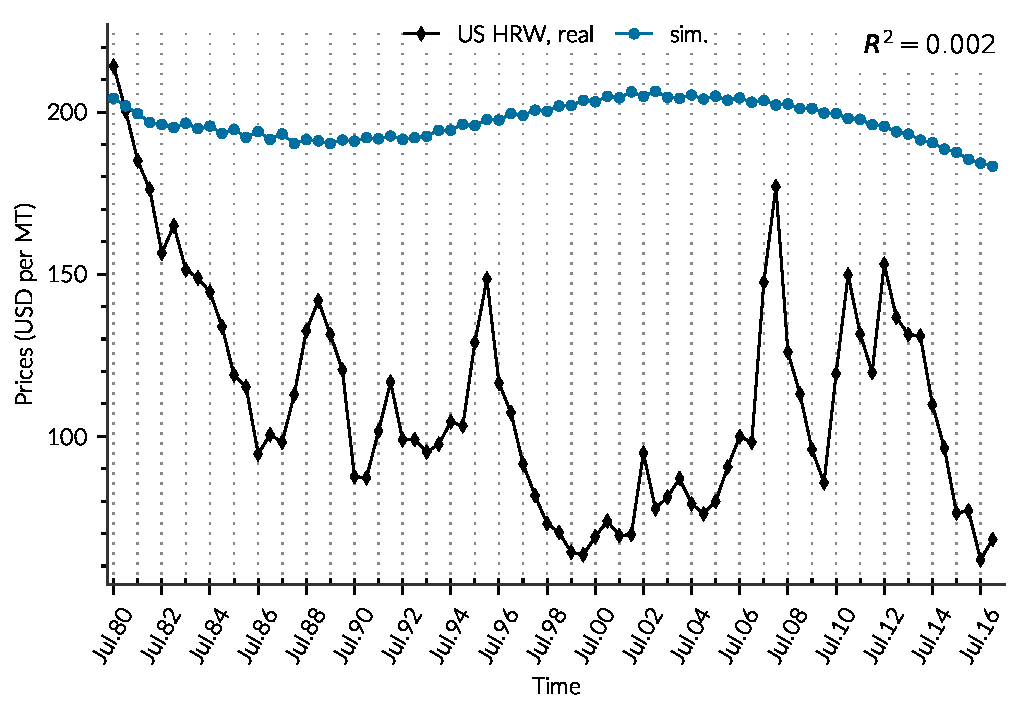
\includegraphics[width=.8\textwidth]{plots/trends_only/pric1980_2017}
\caption{Prices for the scenario accounting only for long-term changes in regional production and
  consumption. Black diamonds and blue dots indicate real and simulated wheat prices,
  respectively. The squared Pearson correlation coefficient $R^2$ denotes the correlation between
  reported and simulated prices. Parameters are as in Tab.~\ref{tab:params}.} %
  \label{fig:trendsOnly}
\end{figure}
\begin{figure}[ht]
  \centering 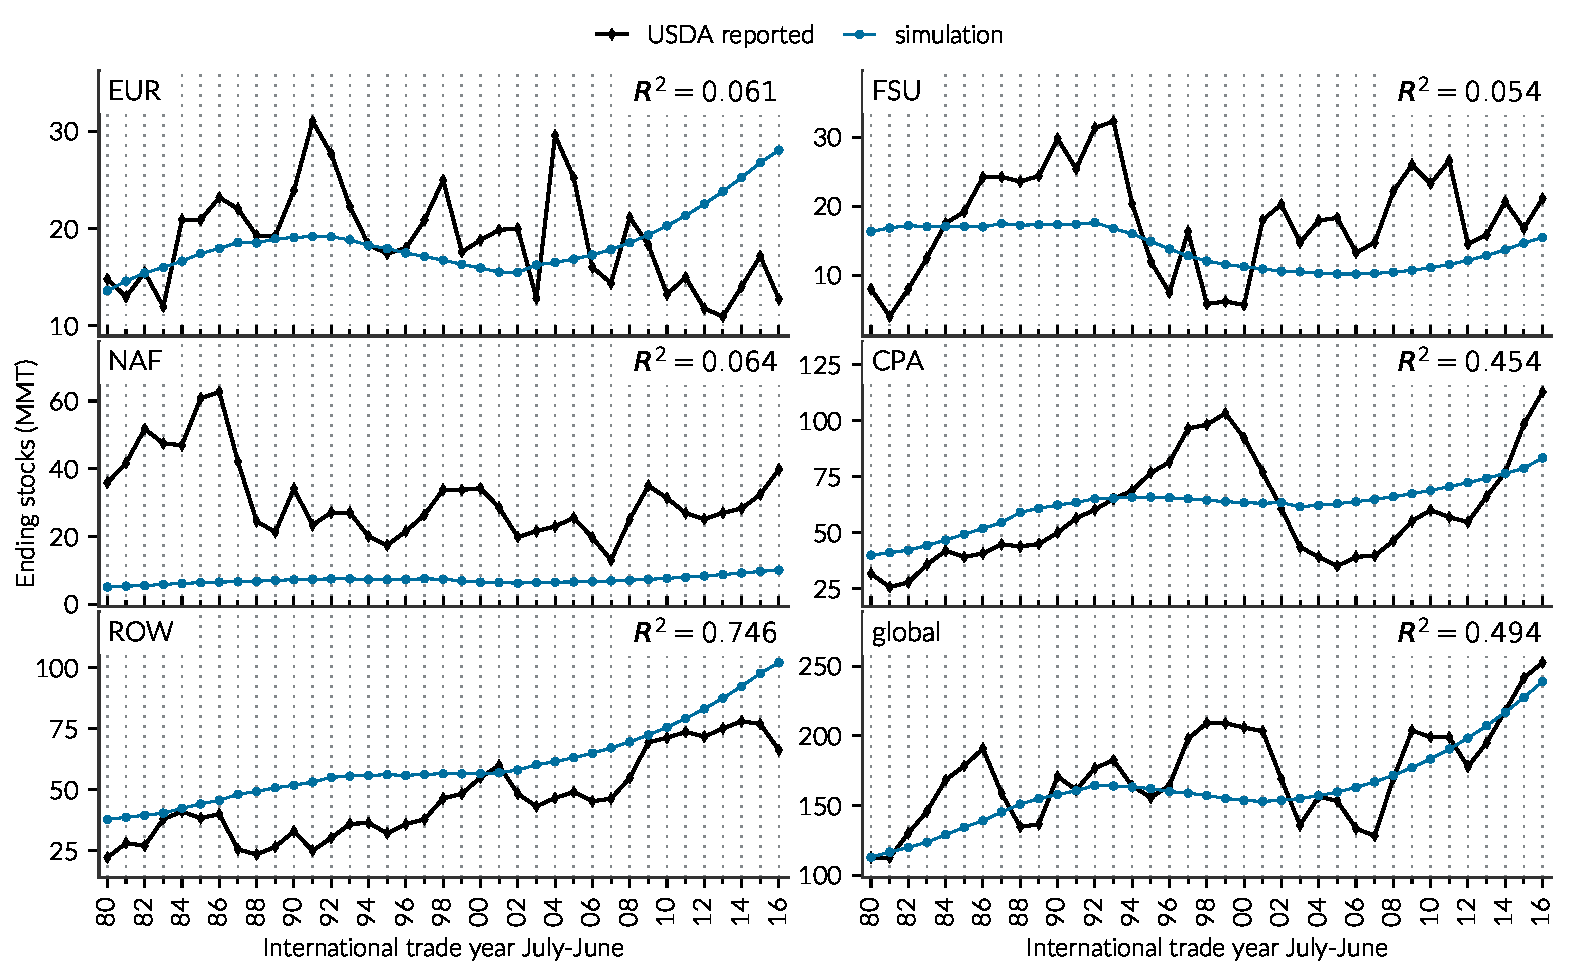
\includegraphics[width=.8\textwidth]{plots/trends_only/Ending_stocks__MMT__1980_2017}
  \caption{Regional ending stock for the scenario accounting only for long-term regional production
    and consumption trends. Reported and simulated ending stocks are denoted by black diamonds and
    blue dots, respectively. Squared Pearson correlation coefficients $R^2$ denote the correlation
    between reported and simulated ending stocks. Regions are the same as in Tab.~\ref{tab:conGroup}.}
  \label{fig:stocks_trendsOnly}
\end{figure}
This scenario accounts only for long-term regional production and consumption trends. As model
input, the smoothed production and domestic consumption time series of
Fig.~\ref{fig:supProd_and_cons} are used. The size of the strategic inventory in each region $r$ are
chosen to be a multiple of the temporal average of the region's mean domestic consumption in the
last three years and its mean expected consumption within the foresight period
$\langle C_r\rangle_{3+1}$ (cf. Eq.~(\ref{eq:Ismaxr})). Since the scenario does not take any
regional policies into account, the same multiple is chosen for all regions.  In the initial steady
state, first $\langle C_r\rangle_{3+1}$ is set to the adjusted domestic regional consumption
described in Sec.~\ref{si:iniCond}. Then, we calculate the global capacity of strategic inventories
$\starIsmax$ by summing Eq.~(\ref{eq:IrmaxIni}) over all regions. The common multiple is then set to
$\starIsmax/\langle C\rangle_{3+1}$, where $\langle C\rangle_{3+1}$ denotes the temporal average of
global domestic consumption.

It is worthy to note that the slight zigzagging of simulated prices in
Fig.~\ref{fig:trendsOnly} results from the finite costs for storage keeping. In this scenario,
expected consumption and world market supply are nearly constant over the foresight periods of the
competitive storage holders. Therefore, the storage holders decide to sell in the first semester of
their local agricultural years more grain on the WM than in the second semester. Because the
majority of wheat is produced in the Northern Hemisphere, more wheat is sold on the WM during the
harvesting season in the Northern Hemisphere (July-December) causing the periodical price drops.


\subsection{Production \& consumption variability}
\begin{figure}[htbp]
  \centering
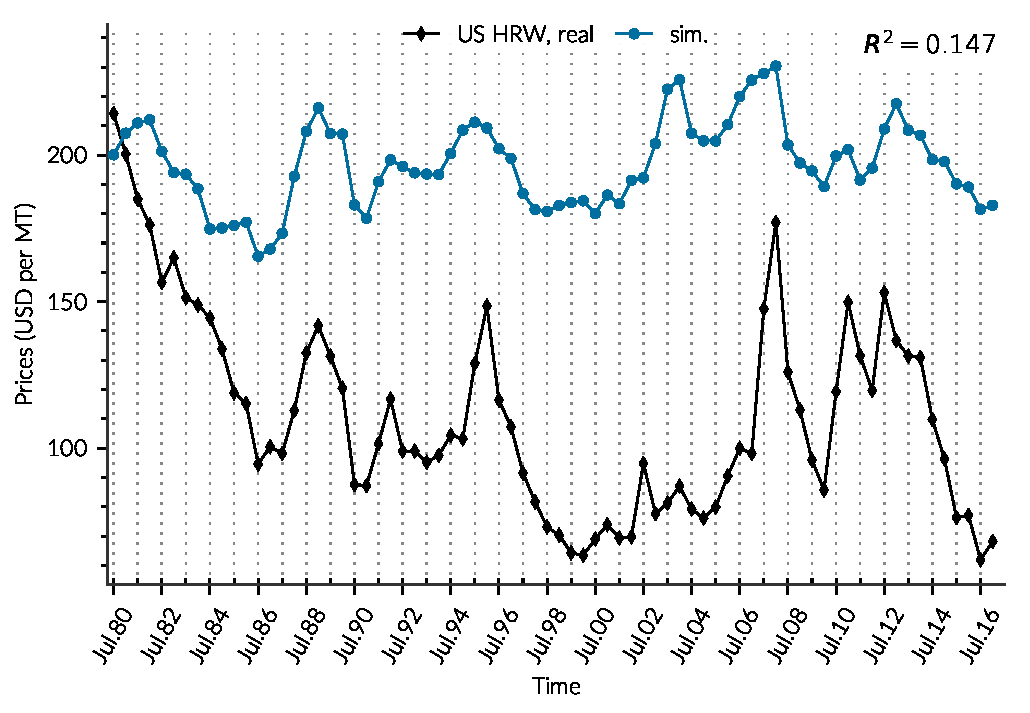
\includegraphics[width=.8\textwidth]{plots/baseline/pric1980_2017}
\caption{Prices for the scenario accounting for regional production and consumption
  variabilities. Black diamonds and blue dots indicate real wheat prices and simulated
  prices, respectively. The squared Pearson correlation coefficient $R^2$ denotes the correlation
  between reported and simulated prices. Parameters are as in Tab.~\ref{tab:params}.} %
  \label{fig:baseline}
\end{figure}
\begin{figure}[htbp]
  \centering 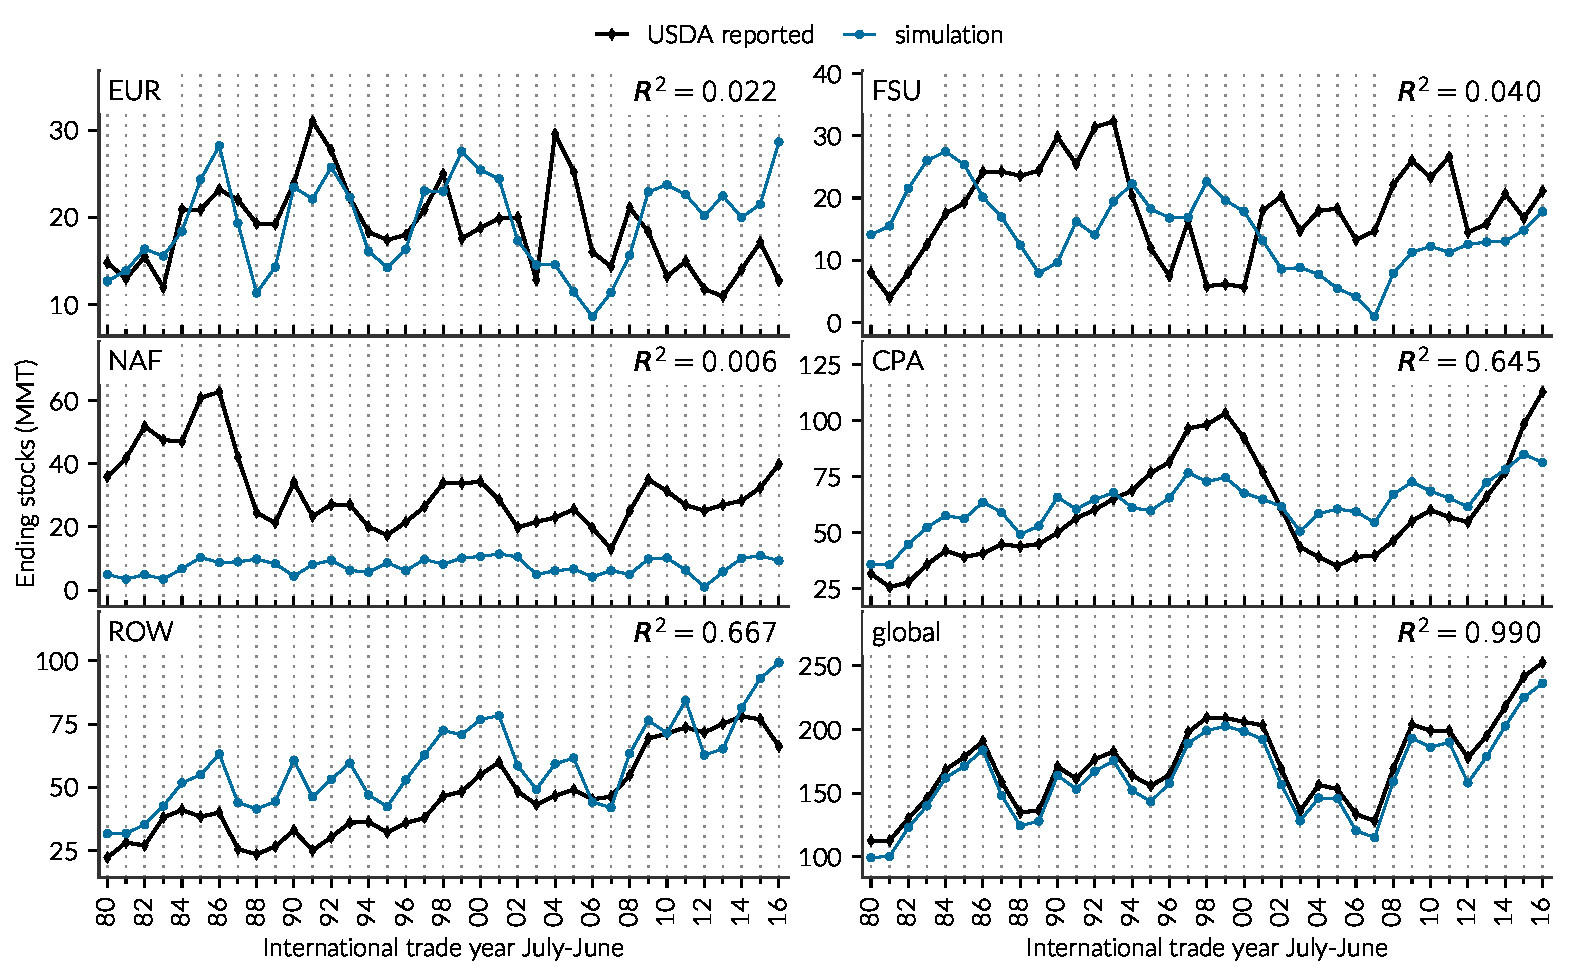
\includegraphics[width=.8\textwidth]{plots/baseline/Ending_stocks__MMT__1980_2017}
  \caption{Regional ending stock for the scenario accounting for production and consumption
    variabilities. Reported and simulated ending stocks are denoted by black diamonds and blue dots,
    respectively. Squared pearson correlation coefficients $R^2$ denote the correlation between
    reported and simulated ending stocks. Regions are the same as in Tab.~\ref{tab:conGroup}.}
  \label{fig:stocks_baseline}
\end{figure}
This scenario accounts for annual variability in production and domestic consumption (see production
and domestic consumption time series in Fig.~\ref{fig:supProd_and_cons}). Since no policies are
taken into account, the size of the strategic inventories are chosen as for the `trends only'
scenario.

% \FloatBarrier

\subsection{No policies from 2006 onwards}
\begin{figure}[htbp]
\centering  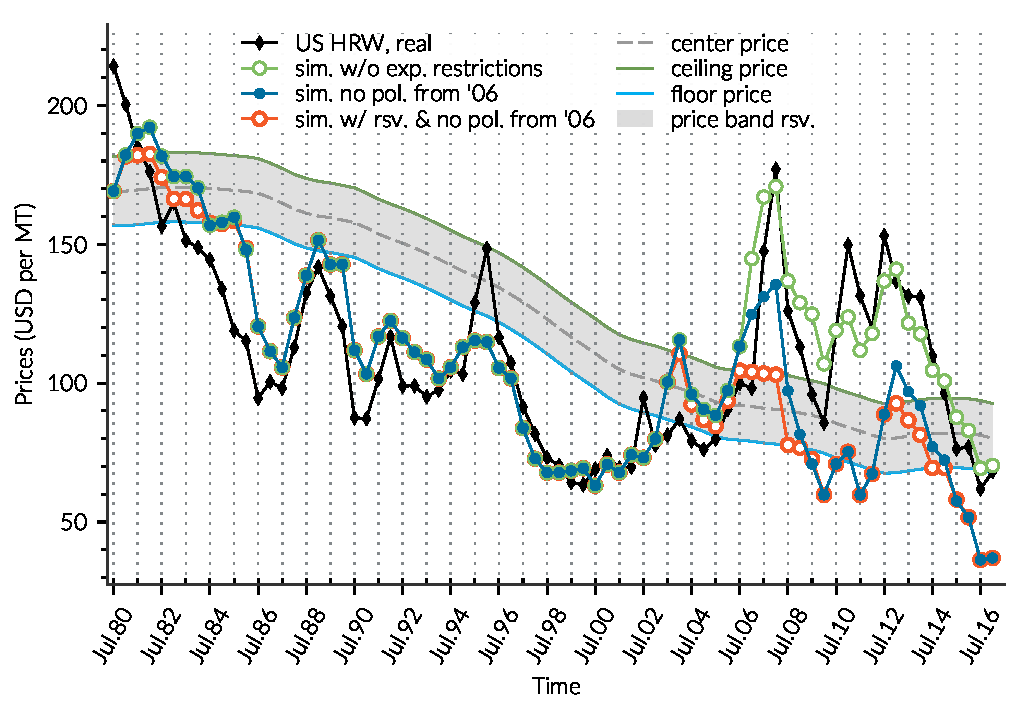
\includegraphics[width=.8\textwidth]{plots/no_policies_after_2006/pric1980_2017}
\caption{Prices for the scenarios without export restrictions and without policy interventions from
  2006 onwards. Black diamonds, green dots, blue dots, and open orange circles indicate real wheat
  prices, simulated prices for the scenario without export restrictions as well as the scenario
  without policy interventions from 2006 onwards (without and with an international reserve with a
  capacity of 30\mmt), respectively. The gray shaded area indicates the price band of the
  international reserve; the reserve is re-stocked (released) if prices drop below (increase above)
  the floor price (thin light-blue line) (ceiling price (thin green line)). The price band has a width of 25\USD~and spans around the 15-years running mean (gray dashed line). Parameters are as in Tab.~\ref{tab:params}.}
  \label{fig:prices_small_res}
\end{figure}
\begin{figure}[htbp]
  \centering 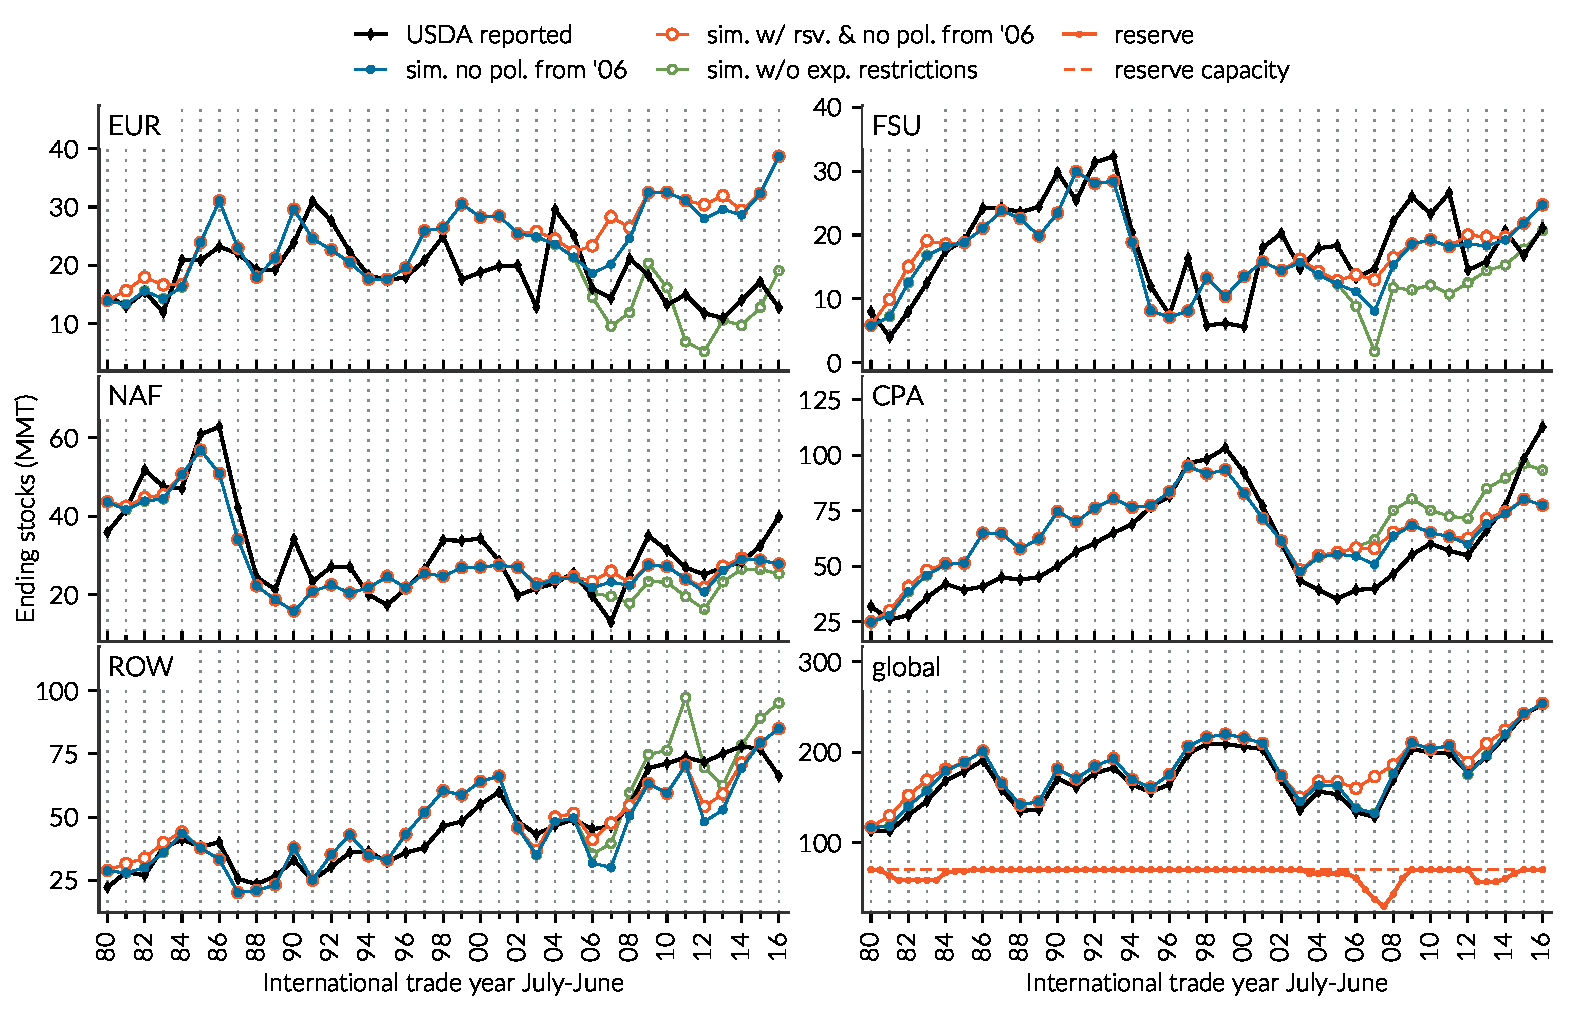
\includegraphics[width=.8\textwidth]{plots/no_policies_after_2006/Ending_stocks__MMT__1980_2017}
  \caption{Regional ending stock for the scenarios of Fig.~\ref{fig:prices_small_res}. Black
    diamonds, open green circles, blue dots, and open orange circles, indicate ending stocks as
    reported by USDA, for the scenario without export restrictions as well as the scenario without
    policy interventions from 2006 onwards (without and with international reserve),
    respectively. Parameters are as in Tab.~\ref{tab:params}. Regions are the same as in Tab.~\ref{tab:conGroup}.}
  \label{fig:stocks_small_res}
\end{figure}
This scenario describes, the optimal outcome of binding free-trade legislation impeding all kinds of
beggar-thy-neighbor policies after 2006. Thus, the factors $\lbrace m_r\rstu_r\rbrace_r$, describing
the regional demand for strategic stock-keeping are fixed to their 2006 levels for the international
trade years 2007 to 2016. Simulated prices and ending stocks resulting from this sceario are
depicted by open open orange circles in Figs.~\ref{fig:prices_small_res} and
\ref{fig:stocks_small_res}, respectively. In this scenario, a reserve of 30\mmt~would have been
sufficient to further mitigate the 2007/08 price spike (see filled open orange circles in
Figs.~\ref{fig:prices_small_res} and \ref{fig:stocks_small_res}). Since no consumption adaptation is
taken into account, the international reserve is initially filled to its capacity (see
discussion in main text.).

Further, the green dots in Figs.~\ref{fig:prices_small_res} and \ref{fig:stocks_small_res} depict a
scenario where only export restrictions are suppressed but the other policies are the same as in the
full historical scenario (cp. Figs.~\ref{fig:Fig1} and \ref{fig:Fig2}).

% \FloatBarrier

\subsection{Iso-elastic regional consumptions}
\begin{figure}[htbp]
  \centering
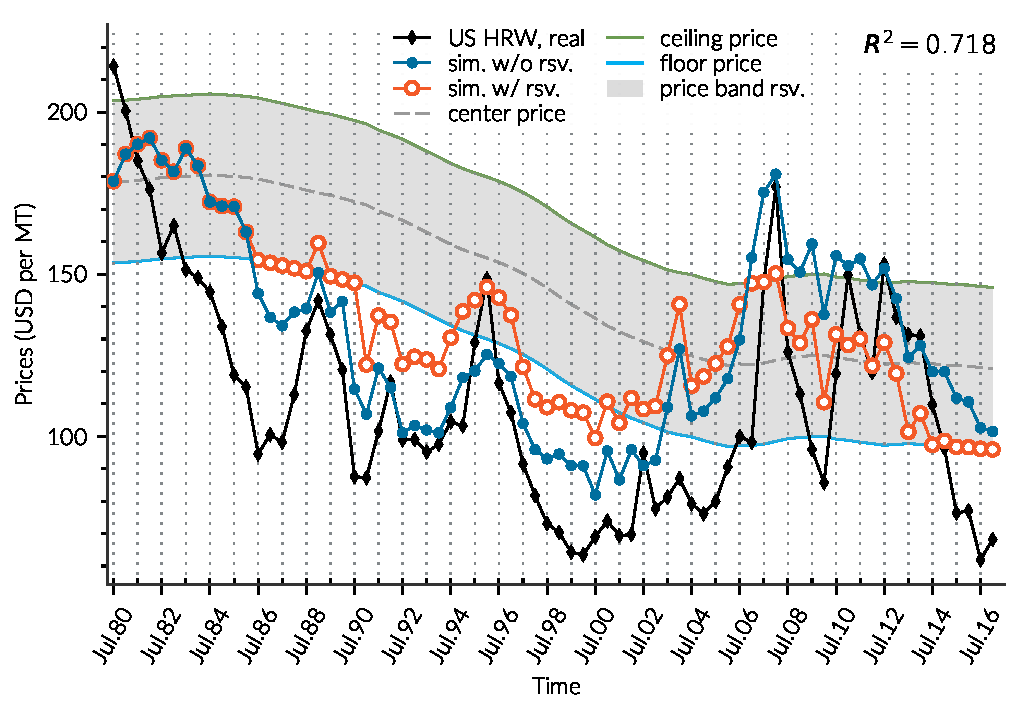
\includegraphics[width=.8\textwidth]{plots/full_var_demand/pric1980_2017}
\caption{Prices for the historical scenario with iso-elastic regional consumptions. Real wheat
  prices (black diamonds), simulated prices without (blue dots), and with a international reserve
  having a capacity of 70\mmt~(open orange circles). The gray shaded area indicates the price band
  of the international reserve; the reserve is re-stocked (released) if prices drop below (increase
  above) the floor price (thin light-blue line) (ceiling price (thin green line)). The price band
  has a width of 55\USD~and spans around the 15-years running mean (gray dashed line). The
  squared Pearson correlation coefficient $R^2$ denotes the correlation between reported prices and
  simulated prices (w/o reserve). Consumption elasticities are $\dce_{\CPA}=-0.1$, $\dce_{\ROW}=-0.05$, $\dce_{\EUR}=-0.15$, $\dce_{\FSU}=-0.5$, and $\dce_{\NAF}=-0.4$, and other parameters are as in
  Tab.~\ref{tab:params}.}
    \label{fig:varDem_price}
\end{figure}
\begin{figure}[htbp]
  \centering 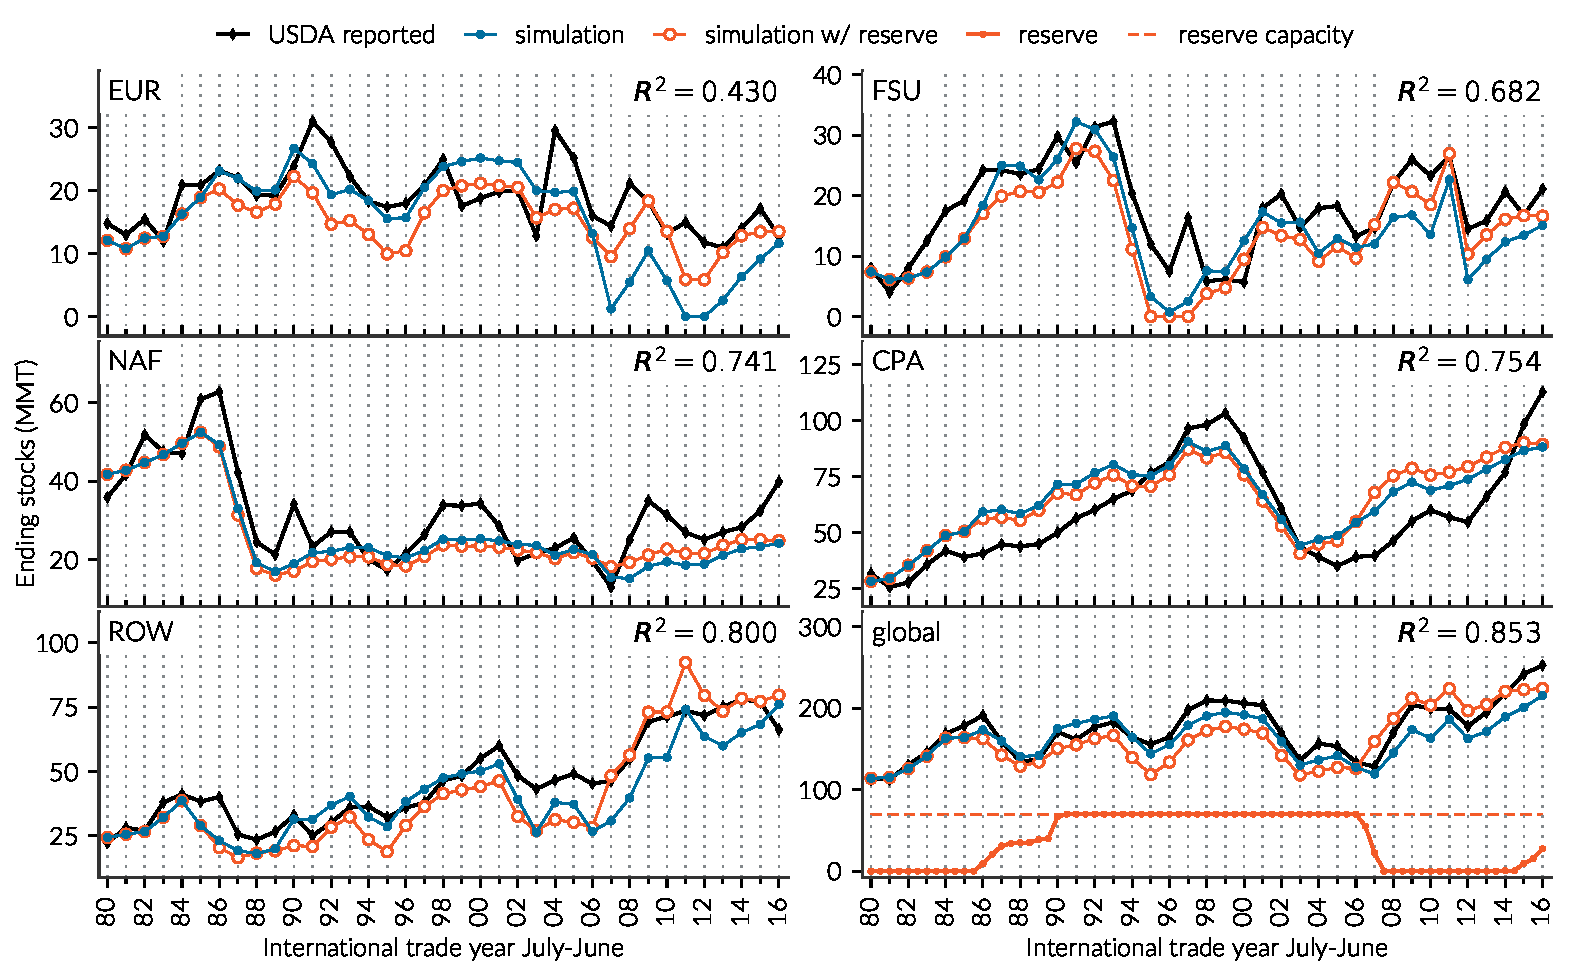
\includegraphics[width=.8\textwidth]{plots/full_var_demand/Ending_stocks__MMT__1980_2017}
  \caption{Regional ending stocks for the historical scenario with iso-elastic regional
    consumptions. Black diamonds, blue dots, and open orange circles, indicate ending stocks as
    reported by USDA, for the scenarios without and with international reserve,
    respectively. Squared Pearson correlation coefficients $R^2$ denote the correlation between
    reported stocks and the scenario without international reserve. Parameters are as in
    Fig.~\ref{fig:varDem_price}. Regions are the same as in Tab.~\ref{tab:conGroup}.}
    \label{fig:varDem_stocks}
\end{figure}
\begin{figure}[htbp]
  \centering  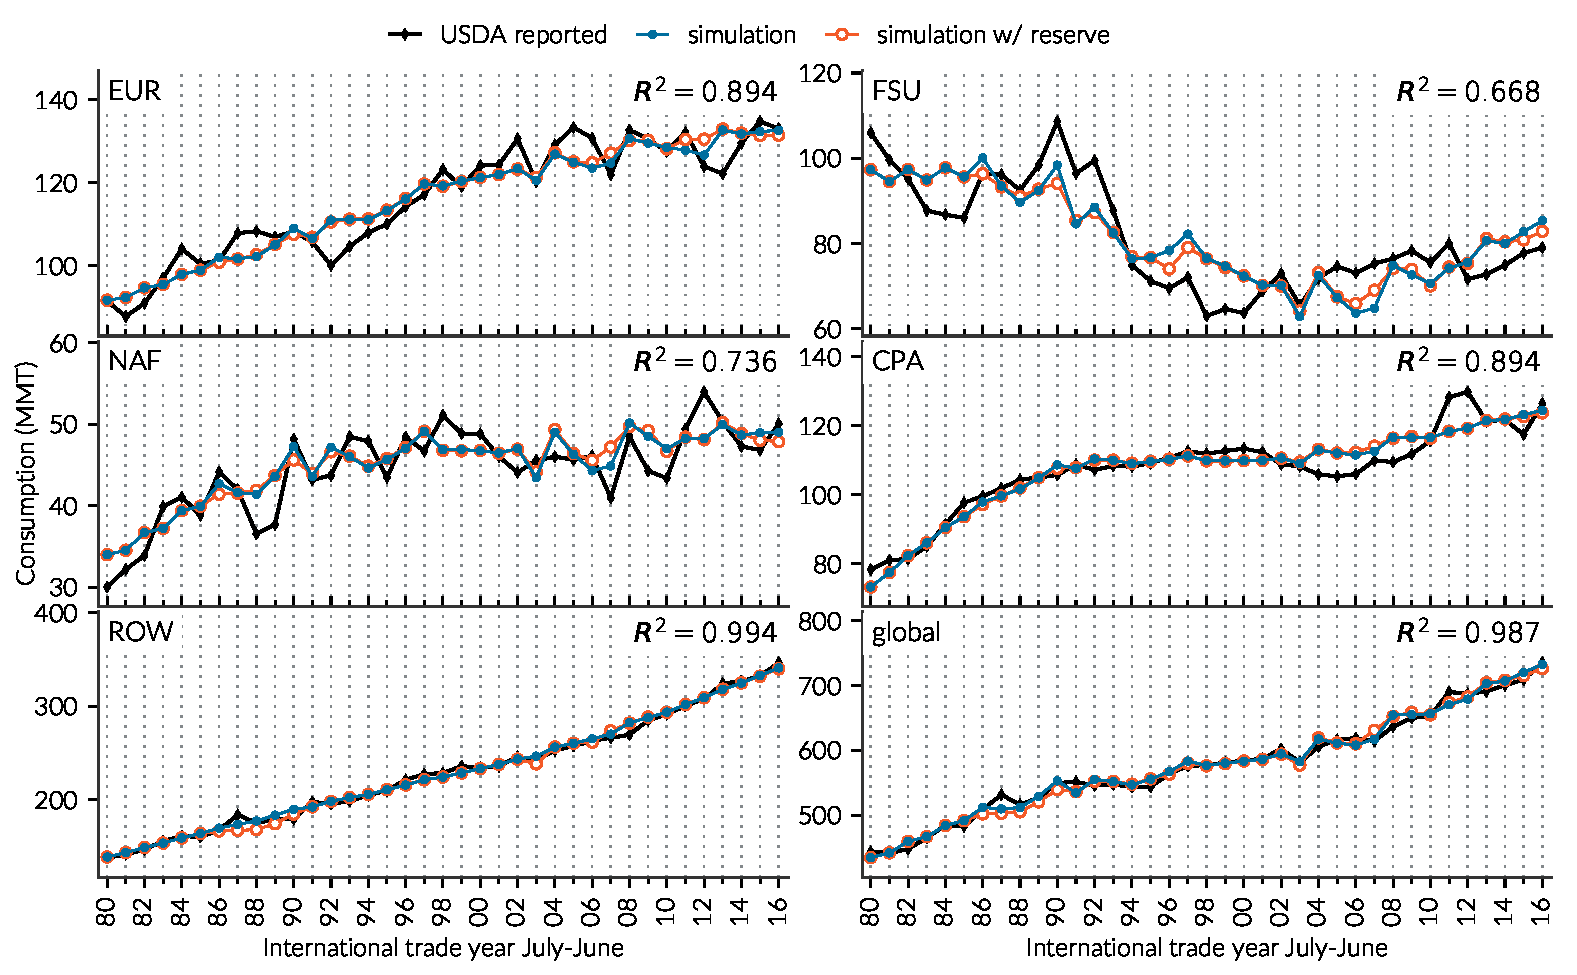
\includegraphics[width=.8\textwidth]{plots/full_var_demand/Consumption__MMT__1980_2017}
  \caption{Regional consumptions for the historical scenario with iso-elastic regional consumption. Color code is the same as in Fig.~\ref{fig:varDem_stocks}. Parameters are as in Fig.~\ref{fig:varDem_price}. Regions are the same as in Tab.~\ref{tab:conGroup}.}
  \label{fig:varDem_cons}
\end{figure}
This scenario corresponds to the full historic scenario described in the main text
(cf. Figs.~\ref{fig:Fig1} and \ref{fig:Fig2})) with the difference that now the regional
consumptions are assumed to depend iso-elastically upon WM price (see
Eq.~(\ref{eq:C_r})). Figures.~\ref{fig:varDem_price} and \ref{fig:varDem_stocks} compare simulated
WM prices and regional ending stocks with reported prices and ending stocks, respectively. The
elasticities of consumption vary among regions, which expresses the regions' different dependencies
upon the modeled crop. They are determined by best fit of simulated regional consumptions with
reported annual regional domestic consumption (see Fig.~\ref{fig:varDem_cons}) as
$\dce_{\CPA}=-0.1$, $\dce_{\ROW}=-0.05$, $\dce_{\EUR}=-0.15$, $\dce_{\FSU}=-0.5$, and $\dce_{\NAF}=-0.4$.  Further,
regional baseline consumption is determined from the average regional consumption of the last 3
years, $\Cref_r\equiv \langle C_r\rangle_3$, and the reference price is determined from the average
WM price of the last 3 years, $\Pref_r\equiv \langle \Pref_r\rangle_2$
(cf. Eq.~(\ref{eq:C_r})). In the initial steady state, the reference prices of all regions are set
to the reported WM price in the first semester of the international trade year.

Since, in this scenario, consumption adaption can be accounted for, the
reserve is chosen to be initially empty. Figure~\ref{fig:varDem_stocks} shows
that the build-up of the reserve has no significant negative impact on regional
endings stocks, and Fig.~\ref{fig:varDem_cons} reveals that regional domestic
consumption is only somewhat reduced. Thus, the negative impact of the reserve's build-up on vulnerable consumers is negligibly small.

% \FloatBarrier

\subsection{Statistical analysis}
\label{sec:artiTs}
This section provides details on the statistical analysis of Fig.~\ref{fig:Fig3}.

\paragraph{Initial conditions}
The simulations are initialized with the average regional productions and ending stocks of the
international trade years 2010 to 2015. Further, we use the average regional consumption of these
years to determine initial regional consumptions as described in Sec.~\ref{si:iniCond}. The initial
sizes of the strategical inventories $\lbrace \Ismax_r\rbrace_r$ are determined as described in
Sec.~\ref{si:iniCond}.

\paragraph{Artificial production time series}
Regional historical production anomalies are derived from USDA regional production data for the
international trade years 1965 to 2016 by de-trending with the smoothed data of Fig.~\ref{fig:supProd_and_cons}. The
artificial regional production time series having a length of 10,000 years are assembled by
randomly drawing, for each year and each region, a production anomaly out of the sample of
historical regional production anomalies. However, the results do not change qualitatively if the
regional anomalies are fitted by normal distributions, and the time series are generated by drawing
samples from these distributions. Further, regional baseline consumption $\Cref_r$ is determined
from the average regional consumption of the last 3 years, $\Cref_r\equiv \langle C_r\rangle_3$
(cf. Eq.~(\ref{eq:C_r})), and the reference price $\Pref_r$ is set to the average observed price of
the international trade years 2010 to 2015.

%%% Local Variables:
%%% mode: latex
%%% TeX-master: "multi_twist.tex"
%%% End:


\end{document}


%%% Local Variables:
%%% mode: latex
%%% TeX-master: t
%%% End:
